\documentclass[a4paper,12pt,twoside]{report}
%%%%% NEW MATH DEFINITIONS %%%%%

\usepackage{amsmath,amsfonts,bm}

% Mark sections of captions for referring to divisions of figures
\newcommand{\figleft}{{\em (Left)}}
\newcommand{\figcenter}{{\em (Center)}}
\newcommand{\figright}{{\em (Right)}}
\newcommand{\figtop}{{\em (Top)}}
\newcommand{\figbottom}{{\em (Bottom)}}
\newcommand{\captiona}{{\em (a)}}
\newcommand{\captionb}{{\em (b)}}
\newcommand{\captionc}{{\em (c)}}
\newcommand{\captiond}{{\em (d)}}

% Highlight a newly defined term
\newcommand{\newterm}[1]{{\bf #1}}


% Figure reference, lower-case.
\def\figref#1{figure~\ref{#1}}
% Figure reference, capital. For start of sentence
\def\Figref#1{Figure~\ref{#1}}
\def\twofigref#1#2{figures \ref{#1} and \ref{#2}}
\def\quadfigref#1#2#3#4{figures \ref{#1}, \ref{#2}, \ref{#3} and \ref{#4}}
% Section reference, lower-case.
\def\secref#1{section~\ref{#1}}
% Section reference, capital.
\def\Secref#1{Section~\ref{#1}}
% Reference to two sections.
\def\twosecrefs#1#2{sections \ref{#1} and \ref{#2}}
% Reference to three sections.
\def\secrefs#1#2#3{sections \ref{#1}, \ref{#2} and \ref{#3}}
% Reference to an equation, lower-case.
\def\eqref#1{equation~\ref{#1}}
% Reference to an equation, upper case
\def\Eqref#1{Equation~\ref{#1}}
% A raw reference to an equation---avoid using if possible
\def\plaineqref#1{\ref{#1}}
% Reference to a chapter, lower-case.
\def\chapref#1{chapter~\ref{#1}}
% Reference to an equation, upper case.
\def\Chapref#1{Chapter~\ref{#1}}
% Reference to a range of chapters
\def\rangechapref#1#2{chapters\ref{#1}--\ref{#2}}
% Reference to an algorithm, lower-case.
\def\algref#1{algorithm~\ref{#1}}
% Reference to an algorithm, upper case.
\def\Algref#1{Algorithm~\ref{#1}}
\def\twoalgref#1#2{algorithms \ref{#1} and \ref{#2}}
\def\Twoalgref#1#2{Algorithms \ref{#1} and \ref{#2}}
% Reference to a part, lower case
\def\partref#1{part~\ref{#1}}
% Reference to a part, upper case
\def\Partref#1{Part~\ref{#1}}
\def\twopartref#1#2{parts \ref{#1} and \ref{#2}}

\def\ceil#1{\lceil #1 \rceil}
\def\floor#1{\lfloor #1 \rfloor}
\def\1{\bm{1}}
\newcommand{\train}{\mathcal{D}}
\newcommand{\valid}{\mathcal{D_{\mathrm{valid}}}}
\newcommand{\test}{\mathcal{D_{\mathrm{test}}}}

\def\eps{{\epsilon}}


% Random variables
\def\reta{{\textnormal{$\eta$}}}
\def\ra{{\textnormal{a}}}
\def\rb{{\textnormal{b}}}
\def\rc{{\textnormal{c}}}
\def\rd{{\textnormal{d}}}
\def\re{{\textnormal{e}}}
\def\rf{{\textnormal{f}}}
\def\rg{{\textnormal{g}}}
\def\rh{{\textnormal{h}}}
\def\ri{{\textnormal{i}}}
\def\rj{{\textnormal{j}}}
\def\rk{{\textnormal{k}}}
\def\rl{{\textnormal{l}}}
% rm is already a command, just don't name any random variables m
\def\rn{{\textnormal{n}}}
\def\ro{{\textnormal{o}}}
\def\rp{{\textnormal{p}}}
\def\rq{{\textnormal{q}}}
\def\rr{{\textnormal{r}}}
\def\rs{{\textnormal{s}}}
\def\rt{{\textnormal{t}}}
\def\ru{{\textnormal{u}}}
\def\rv{{\textnormal{v}}}
\def\rw{{\textnormal{w}}}
\def\rx{{\textnormal{x}}}
\def\ry{{\textnormal{y}}}
\def\rz{{\textnormal{z}}}

% Random vectors
\def\rvepsilon{{\mathbf{\epsilon}}}
\def\rvtheta{{\mathbf{\theta}}}
\def\rva{{\mathbf{a}}}
\def\rvb{{\mathbf{b}}}
\def\rvc{{\mathbf{c}}}
\def\rvd{{\mathbf{d}}}
\def\rve{{\mathbf{e}}}
\def\rvf{{\mathbf{f}}}
\def\rvg{{\mathbf{g}}}
\def\rvh{{\mathbf{h}}}
\def\rvu{{\mathbf{i}}}
\def\rvj{{\mathbf{j}}}
\def\rvk{{\mathbf{k}}}
\def\rvl{{\mathbf{l}}}
\def\rvm{{\mathbf{m}}}
\def\rvn{{\mathbf{n}}}
\def\rvo{{\mathbf{o}}}
\def\rvp{{\mathbf{p}}}
\def\rvq{{\mathbf{q}}}
\def\rvr{{\mathbf{r}}}
\def\rvs{{\mathbf{s}}}
\def\rvt{{\mathbf{t}}}
\def\rvu{{\mathbf{u}}}
\def\rvv{{\mathbf{v}}}
\def\rvw{{\mathbf{w}}}
\def\rvx{{\mathbf{x}}}
\def\rvy{{\mathbf{y}}}
\def\rvz{{\mathbf{z}}}

% Elements of random vectors
\def\erva{{\textnormal{a}}}
\def\ervb{{\textnormal{b}}}
\def\ervc{{\textnormal{c}}}
\def\ervd{{\textnormal{d}}}
\def\erve{{\textnormal{e}}}
\def\ervf{{\textnormal{f}}}
\def\ervg{{\textnormal{g}}}
\def\ervh{{\textnormal{h}}}
\def\ervi{{\textnormal{i}}}
\def\ervj{{\textnormal{j}}}
\def\ervk{{\textnormal{k}}}
\def\ervl{{\textnormal{l}}}
\def\ervm{{\textnormal{m}}}
\def\ervn{{\textnormal{n}}}
\def\ervo{{\textnormal{o}}}
\def\ervp{{\textnormal{p}}}
\def\ervq{{\textnormal{q}}}
\def\ervr{{\textnormal{r}}}
\def\ervs{{\textnormal{s}}}
\def\ervt{{\textnormal{t}}}
\def\ervu{{\textnormal{u}}}
\def\ervv{{\textnormal{v}}}
\def\ervw{{\textnormal{w}}}
\def\ervx{{\textnormal{x}}}
\def\ervy{{\textnormal{y}}}
\def\ervz{{\textnormal{z}}}

% Random matrices
\def\rmA{{\mathbf{A}}}
\def\rmB{{\mathbf{B}}}
\def\rmC{{\mathbf{C}}}
\def\rmD{{\mathbf{D}}}
\def\rmE{{\mathbf{E}}}
\def\rmF{{\mathbf{F}}}
\def\rmG{{\mathbf{G}}}
\def\rmH{{\mathbf{H}}}
\def\rmI{{\mathbf{I}}}
\def\rmJ{{\mathbf{J}}}
\def\rmK{{\mathbf{K}}}
\def\rmL{{\mathbf{L}}}
\def\rmM{{\mathbf{M}}}
\def\rmN{{\mathbf{N}}}
\def\rmO{{\mathbf{O}}}
\def\rmP{{\mathbf{P}}}
\def\rmQ{{\mathbf{Q}}}
\def\rmR{{\mathbf{R}}}
\def\rmS{{\mathbf{S}}}
\def\rmT{{\mathbf{T}}}
\def\rmU{{\mathbf{U}}}
\def\rmV{{\mathbf{V}}}
\def\rmW{{\mathbf{W}}}
\def\rmX{{\mathbf{X}}}
\def\rmY{{\mathbf{Y}}}
\def\rmZ{{\mathbf{Z}}}

% Elements of random matrices
\def\ermA{{\textnormal{A}}}
\def\ermB{{\textnormal{B}}}
\def\ermC{{\textnormal{C}}}
\def\ermD{{\textnormal{D}}}
\def\ermE{{\textnormal{E}}}
\def\ermF{{\textnormal{F}}}
\def\ermG{{\textnormal{G}}}
\def\ermH{{\textnormal{H}}}
\def\ermI{{\textnormal{I}}}
\def\ermJ{{\textnormal{J}}}
\def\ermK{{\textnormal{K}}}
\def\ermL{{\textnormal{L}}}
\def\ermM{{\textnormal{M}}}
\def\ermN{{\textnormal{N}}}
\def\ermO{{\textnormal{O}}}
\def\ermP{{\textnormal{P}}}
\def\ermQ{{\textnormal{Q}}}
\def\ermR{{\textnormal{R}}}
\def\ermS{{\textnormal{S}}}
\def\ermT{{\textnormal{T}}}
\def\ermU{{\textnormal{U}}}
\def\ermV{{\textnormal{V}}}
\def\ermW{{\textnormal{W}}}
\def\ermX{{\textnormal{X}}}
\def\ermY{{\textnormal{Y}}}
\def\ermZ{{\textnormal{Z}}}

% Vectors
\def\vzero{{\bm{0}}}
\def\vone{{\bm{1}}}
\def\vmu{{\bm{\mu}}}
\def\vtheta{{\bm{\theta}}}
\def\va{{\bm{a}}}
\def\vb{{\bm{b}}}
\def\vc{{\bm{c}}}
\def\vd{{\bm{d}}}
\def\ve{{\bm{e}}}
\def\vf{{\bm{f}}}
\def\vg{{\bm{g}}}
\def\vh{{\bm{h}}}
\def\vi{{\bm{i}}}
\def\vj{{\bm{j}}}
\def\vk{{\bm{k}}}
\def\vl{{\bm{l}}}
\def\vm{{\bm{m}}}
\def\vn{{\bm{n}}}
\def\vo{{\bm{o}}}
\def\vp{{\bm{p}}}
\def\vq{{\bm{q}}}
\def\vr{{\bm{r}}}
\def\vs{{\bm{s}}}
\def\vt{{\bm{t}}}
\def\vu{{\bm{u}}}
\def\vv{{\bm{v}}}
\def\vw{{\bm{w}}}
\def\vx{{\bm{x}}}
\def\vy{{\bm{y}}}
\def\vz{{\bm{z}}}

% Elements of vectors
\def\evalpha{{\alpha}}
\def\evbeta{{\beta}}
\def\evepsilon{{\epsilon}}
\def\evlambda{{\lambda}}
\def\evomega{{\omega}}
\def\evmu{{\mu}}
\def\evpsi{{\psi}}
\def\evsigma{{\sigma}}
\def\evtheta{{\theta}}
\def\eva{{a}}
\def\evb{{b}}
\def\evc{{c}}
\def\evd{{d}}
\def\eve{{e}}
\def\evf{{f}}
\def\evg{{g}}
\def\evh{{h}}
\def\evi{{i}}
\def\evj{{j}}
\def\evk{{k}}
\def\evl{{l}}
\def\evm{{m}}
\def\evn{{n}}
\def\evo{{o}}
\def\evp{{p}}
\def\evq{{q}}
\def\evr{{r}}
\def\evs{{s}}
\def\evt{{t}}
\def\evu{{u}}
\def\evv{{v}}
\def\evw{{w}}
\def\evx{{x}}
\def\evy{{y}}
\def\evz{{z}}

% Matrix
\def\mA{{\bm{A}}}
\def\mB{{\bm{B}}}
\def\mC{{\bm{C}}}
\def\mD{{\bm{D}}}
\def\mE{{\bm{E}}}
\def\mF{{\bm{F}}}
\def\mG{{\bm{G}}}
\def\mH{{\bm{H}}}
\def\mI{{\bm{I}}}
\def\mJ{{\bm{J}}}
\def\mK{{\bm{K}}}
\def\mL{{\bm{L}}}
\def\mM{{\bm{M}}}
\def\mN{{\bm{N}}}
\def\mO{{\bm{O}}}
\def\mP{{\bm{P}}}
\def\mQ{{\bm{Q}}}
\def\mR{{\bm{R}}}
\def\mS{{\bm{S}}}
\def\mT{{\bm{T}}}
\def\mU{{\bm{U}}}
\def\mV{{\bm{V}}}
\def\mW{{\bm{W}}}
\def\mX{{\bm{X}}}
\def\mY{{\bm{Y}}}
\def\mZ{{\bm{Z}}}
\def\mBeta{{\bm{\beta}}}
\def\mPhi{{\bm{\Phi}}}
\def\mLambda{{\bm{\Lambda}}}
\def\mSigma{{\bm{\Sigma}}}

% Tensor
\DeclareMathAlphabet{\mathsfit}{\encodingdefault}{\sfdefault}{m}{sl}
\SetMathAlphabet{\mathsfit}{bold}{\encodingdefault}{\sfdefault}{bx}{n}
\newcommand{\tens}[1]{\bm{\mathsfit{#1}}}
\def\tA{{\tens{A}}}
\def\tB{{\tens{B}}}
\def\tC{{\tens{C}}}
\def\tD{{\tens{D}}}
\def\tE{{\tens{E}}}
\def\tF{{\tens{F}}}
\def\tG{{\tens{G}}}
\def\tH{{\tens{H}}}
\def\tI{{\tens{I}}}
\def\tJ{{\tens{J}}}
\def\tK{{\tens{K}}}
\def\tL{{\tens{L}}}
\def\tM{{\tens{M}}}
\def\tN{{\tens{N}}}
\def\tO{{\tens{O}}}
\def\tP{{\tens{P}}}
\def\tQ{{\tens{Q}}}
\def\tR{{\tens{R}}}
\def\tS{{\tens{S}}}
\def\tT{{\tens{T}}}
\def\tU{{\tens{U}}}
\def\tV{{\tens{V}}}
\def\tW{{\tens{W}}}
\def\tX{{\tens{X}}}
\def\tY{{\tens{Y}}}
\def\tZ{{\tens{Z}}}


% Graph
\def\gA{{\mathcal{A}}}
\def\gB{{\mathcal{B}}}
\def\gC{{\mathcal{C}}}
\def\gD{{\mathcal{D}}}
\def\gE{{\mathcal{E}}}
\def\gF{{\mathcal{F}}}
\def\gG{{\mathcal{G}}}
\def\gH{{\mathcal{H}}}
\def\gI{{\mathcal{I}}}
\def\gJ{{\mathcal{J}}}
\def\gK{{\mathcal{K}}}
\def\gL{{\mathcal{L}}}
\def\gM{{\mathcal{M}}}
\def\gN{{\mathcal{N}}}
\def\gO{{\mathcal{O}}}
\def\gP{{\mathcal{P}}}
\def\gQ{{\mathcal{Q}}}
\def\gR{{\mathcal{R}}}
\def\gS{{\mathcal{S}}}
\def\gT{{\mathcal{T}}}
\def\gU{{\mathcal{U}}}
\def\gV{{\mathcal{V}}}
\def\gW{{\mathcal{W}}}
\def\gX{{\mathcal{X}}}
\def\gY{{\mathcal{Y}}}
\def\gZ{{\mathcal{Z}}}

% Sets
\def\sA{{\mathbb{A}}}
\def\sB{{\mathbb{B}}}
\def\sC{{\mathbb{C}}}
\def\sD{{\mathbb{D}}}
% Don't use a set called E, because this would be the same as our symbol
% for expectation.
\def\sF{{\mathbb{F}}}
\def\sG{{\mathbb{G}}}
\def\sH{{\mathbb{H}}}
\def\sI{{\mathbb{I}}}
\def\sJ{{\mathbb{J}}}
\def\sK{{\mathbb{K}}}
\def\sL{{\mathbb{L}}}
\def\sM{{\mathbb{M}}}
\def\sN{{\mathbb{N}}}
\def\sO{{\mathbb{O}}}
\def\sP{{\mathbb{P}}}
\def\sQ{{\mathbb{Q}}}
\def\sR{{\mathbb{R}}}
\def\sS{{\mathbb{S}}}
\def\sT{{\mathbb{T}}}
\def\sU{{\mathbb{U}}}
\def\sV{{\mathbb{V}}}
\def\sW{{\mathbb{W}}}
\def\sX{{\mathbb{X}}}
\def\sY{{\mathbb{Y}}}
\def\sZ{{\mathbb{Z}}}

% Entries of a matrix
\def\emLambda{{\Lambda}}
\def\emA{{A}}
\def\emB{{B}}
\def\emC{{C}}
\def\emD{{D}}
\def\emE{{E}}
\def\emF{{F}}
\def\emG{{G}}
\def\emH{{H}}
\def\emI{{I}}
\def\emJ{{J}}
\def\emK{{K}}
\def\emL{{L}}
\def\emM{{M}}
\def\emN{{N}}
\def\emO{{O}}
\def\emP{{P}}
\def\emQ{{Q}}
\def\emR{{R}}
\def\emS{{S}}
\def\emT{{T}}
\def\emU{{U}}
\def\emV{{V}}
\def\emW{{W}}
\def\emX{{X}}
\def\emY{{Y}}
\def\emZ{{Z}}
\def\emSigma{{\Sigma}}

% entries of a tensor
% Same font as tensor, without \bm wrapper
\newcommand{\etens}[1]{\mathsfit{#1}}
\def\etLambda{{\etens{\Lambda}}}
\def\etA{{\etens{A}}}
\def\etB{{\etens{B}}}
\def\etC{{\etens{C}}}
\def\etD{{\etens{D}}}
\def\etE{{\etens{E}}}
\def\etF{{\etens{F}}}
\def\etG{{\etens{G}}}
\def\etH{{\etens{H}}}
\def\etI{{\etens{I}}}
\def\etJ{{\etens{J}}}
\def\etK{{\etens{K}}}
\def\etL{{\etens{L}}}
\def\etM{{\etens{M}}}
\def\etN{{\etens{N}}}
\def\etO{{\etens{O}}}
\def\etP{{\etens{P}}}
\def\etQ{{\etens{Q}}}
\def\etR{{\etens{R}}}
\def\etS{{\etens{S}}}
\def\etT{{\etens{T}}}
\def\etU{{\etens{U}}}
\def\etV{{\etens{V}}}
\def\etW{{\etens{W}}}
\def\etX{{\etens{X}}}
\def\etY{{\etens{Y}}}
\def\etZ{{\etens{Z}}}

% The true underlying data generating distribution
\newcommand{\pdata}{p_{\rm{data}}}
% The empirical distribution defined by the training set
\newcommand{\ptrain}{\hat{p}_{\rm{data}}}
\newcommand{\Ptrain}{\hat{P}_{\rm{data}}}
% The model distribution
\newcommand{\pmodel}{p_{\rm{model}}}
\newcommand{\Pmodel}{P_{\rm{model}}}
\newcommand{\ptildemodel}{\tilde{p}_{\rm{model}}}
% Stochastic autoencoder distributions
\newcommand{\pencode}{p_{\rm{encoder}}}
\newcommand{\pdecode}{p_{\rm{decoder}}}
\newcommand{\precons}{p_{\rm{reconstruct}}}

\newcommand{\laplace}{\mathrm{Laplace}} % Laplace distribution

\newcommand{\E}{\mathbb{E}}
\newcommand{\Ls}{\mathcal{L}}
\newcommand{\R}{\mathbb{R}}
\newcommand{\emp}{\tilde{p}}
\newcommand{\lr}{\alpha}
\newcommand{\reg}{\lambda}
\newcommand{\rect}{\mathrm{rectifier}}
\newcommand{\softmax}{\mathrm{softmax}}
\newcommand{\sigmoid}{\sigma}
\newcommand{\softplus}{\zeta}
\newcommand{\KL}{D_{\mathrm{KL}}}
\newcommand{\Var}{\mathrm{Var}}
\newcommand{\standarderror}{\mathrm{SE}}
\newcommand{\Cov}{\mathrm{Cov}}
% Wolfram Mathworld says $L^2$ is for function spaces and $\ell^2$ is for vectors
% But then they seem to use $L^2$ for vectors throughout the site, and so does
% wikipedia.
\newcommand{\normlzero}{L^0}
\newcommand{\normlone}{L^1}
\newcommand{\normltwo}{L^2}
\newcommand{\normlp}{L^p}
\newcommand{\normmax}{L^\infty}

\newcommand{\parents}{Pa} % See usage in notation.tex. Chosen to match Daphne's book.

\DeclareMathOperator*{\argmax}{arg\,max}
\DeclareMathOperator*{\argmin}{arg\,min}

\DeclareMathOperator{\sign}{sign}
\DeclareMathOperator{\Tr}{Tr}
\let\ab\allowbreak
 % math commands from https://github.com/goodfeli/dlbook_notation
\usepackage{acronym}
\usepackage{url}
\usepackage{cite}
\usepackage{listings}
\usepackage[pdftex]{graphicx}
\usepackage[hang,small,bf]{caption}
\usepackage{styles/tum}
\usepackage{setspace}
\usepackage[german,english]{babel}
\usepackage{float}
\usepackage{floatflt}
\usepackage{fancyhdr}
\usepackage{color}
\usepackage{booktabs}
\usepackage[pdftex,bookmarks=true,plainpages=false,pdfpagelabels=true]{hyperref}	%TODO make yourself familiar with \label, \ref and \hyperref for referencing figures, tables, chapters, etc.
\usepackage{mdwlist}
\usepackage{enumerate}
\usepackage{array}
\usepackage{longtable}
\usepackage[utf8]{inputenc}
\usepackage{wasysym}
\usepackage[capitalize, noabbrev]{cleveref}

\usepackage[numbers]{natbib}

\usepackage{svg}
\usepackage{amsmath}

\usepackage{subcaption}

\usepackage{algorithm, algorithmic}%

% Path for graphics
\graphicspath{{figures/}}

\begin{document}
\setlength{\evensidemargin}{22pt}
\setlength{\oddsidemargin}{22pt}

\def\doctype{Bachelor's Thesis}
\def\faculty{Informatik}
\def\title{Perceptual Losses for Deep Learning on Fluid Simulations}		%TODO add title in English
\def\titleGer{Perceptual Losses für Deep Learning von Flüssigkeitssimulationen}	%TODO add title in German
\def\supervisor{Prof.\ Dr.\  Nils Thürey}
\def\advisor{M.Sc.\ Georg Kohl}
\def\author{Hanfeng Wu}			%TODO add author name
\def\date{15.09.2021}		%TODO add submission / handover date


\hypersetup{pdfborder={0 0 0},
                        pdfauthor={<author>},
                        pdftitle={thesis-ba-hanfeng},
                        }

\lstset{showspaces=false, numbers=left, frame=single, basicstyle=\small}

\pagenumbering{alph}

\thispagestyle{empty}

\vspace{4cm}
\begin{center}
\begin{figure}[h!]
    \centering
    
\includegraphics[width=4cm]{TUM_Logo_blau_rgb_p}
\end{figure}
\vspace{5mm}     
\huge FAKULT{\"A}T F{\"U}R INFORMATIK\\ 
\vspace{0.5cm}
\large DER TECHNISCHEN UNIVERSIT{\"A}T M{\"U}NCHEN\\
\vspace{1mm}
\end{center}

\vspace{2mm}

\begin{center}
{\Large \doctype\ in \faculty}
\vspace{10mm}

\begin{spacing}{1.5}
{\huge\bf \title}\\%[3ex]
\end{spacing}

\vspace{10mm}
{\LARGE \author}

\vspace{10mm}

\begin{figure}[h!]
\centering
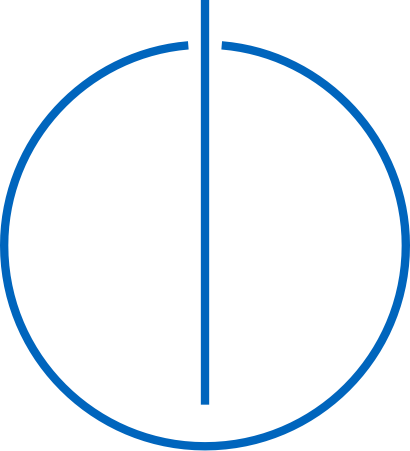
\includegraphics[width=2cm]{FAK_IN_RGB_p}
\end{figure}

\end{center}

\thispagestyle{empty}

\vspace{8mm}
\begin{center}
\oTUM{4cm}

\vspace{5mm}     
\huge FAKULT{\"A}T F{\"U}R INFORMATIK\\ 
\vspace{0.5cm}
\large DER TECHNISCHEN UNIVERSIT{\"A}T M{\"U}NCHEN\\
\end{center}

\vspace{5mm}

\begin{center}
{\Large \doctype\ in \faculty}
\vspace{8mm}

\begin{spacing}{1.3}
{\LARGE \title}\\
\vspace{8mm}

{\LARGE \titleGer}\\
\vspace{8mm}
\end{spacing}

\begin{tabular}{ll}
\Large Author:     & \Large \author     \\[2mm]
\Large Supervisor: & \Large \supervisor \\[2mm]				
\Large Advisor:	   & \Large \advisor    \\[2mm]
\Large Date:       & \Large \date
\end{tabular}

\vspace{1mm}

\begin{figure}[hb!]
\centering
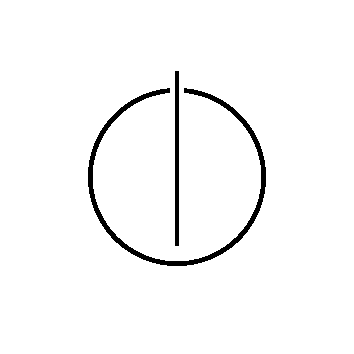
\includegraphics[width=3cm]{InformaticsLogo}
\end{figure}

\end{center}
\newpage
\thispagestyle{empty}
\mbox{}
\clearpage
\thispagestyle{empty}
\vspace*{0.8\textheight}
\noindent
I confirm that this bachelor's thesis is my own work and I have documented all sources and material used.

\vspace{15mm}
\noindent
Munich, \date \hspace{\stretch{1}} \author
\newpage

		%TODO choose one of 'diploma | bachelor's | master's thesis' in the disclaimer file

\newpage
\thispagestyle{empty}
\mbox{}

\chapter*{Acknowledgements}
First I want to thank Prof.\ Nils\ Thürey and my advisor Georg\ Kohl, who offered me this great opportunity to work on this interesting topic. They both have inspired me a lot in this 4-month journey. I also want to thank Prof.\  Kiwon\ Um, who provided me the primitive code of the Solver in the Loop project and helped me to understand the project better. Without the help from anyone of them, I wouldn't have accomplished this thesis.


\pagenumbering{roman}

\selectlanguage{english}
\begin{abstract}

%abstract english

This thesis studies the integration of perceptual losses into several methods or approaches that are related to fluid simulation. Perceptual losses are used to compare high level differences, while traditional loss functions can only compute pixel-level differences reliably. 

First, some general concepts of fluid simulations, deep learning are discussed. Afterwards previous work on perceptual losses is discussed, which mainly focuses on image-related tasks like \cite{johnson2016perceptual, amirshahi2016, berardino2017, bosse2016, kang2014, kim2017}. Next, common methods for data comparison, which is an essential aspect of every perceptual loss function, are compared and characteristics highlighted. Next, we explain in detail several tasks we focus on such as Solver in the Loop and super-resolution. Then, in the experiments we integrate perceptual losses into these tasks in order to show that in the context of fluid simulation, the integration of some pretrained perceptual losses should outperform the traditional loss functions.

Eventually we combine the results of Solver in the Loop and super-resolution models together to achieve a lower time cost comparing to running a traditional fluid simulation.

\end{abstract}

\clearpage

\selectlanguage{german}
\begin{abstract}

Diese Arbeit untersucht die Integration von Percaptual Losses in verschiedene
Methoden oder Ansätze, die im Zusammenhang mit Fluidsimulationen stehen.
Perceptual Losses werden verwendet, um großflächige Unterschiede zu
vergleichen, während herkömmliche Loss Funktionen nur Unterschiede auf
Pixelebene zuverlässig berechnen können.

Zunächst werden einige allgemeine Konzepte von Fluidsimulationen und
Deep Learning erläutert. Anschließend werden bisherige Publikationen zu Perceptual Losses
diskutiert, die sich hauptsächlich auf Aufgaben aus der Bildverarbeitung konzentrieren, wie etwa  \cite{johnson2016perceptual, amirshahi2016, berardino2017, bosse2016, kang2014, kim2017}. Als nächstes werden gängie Methoden
für den Datenvergleich, der ein wesentlicher Aspekt jedes Perceptual Losses
ist, verglichen und deren Eigenschaften hervorgehoben. Danach
erklären wir detailiert die verschiedenen Aufgaben auf die wir uns konzentrieren,
wie Solver in the Loop und super-resolution. Dann integrieren wir in den Experimenten Perceptual Losses in diese Aufgaben, um zu zeigen, dass
im Kontext von Fluidsimulation die Integration einiger Perceptual Losses traditionelle
Formulierungen von Losses übertrifft.

Abschließend kombinieren wir die Ergebnisse von den Modellen für Solver in the Loop und
super-resolution, um im Vergleich zu einer herkömmlichen Fluidsimulation
eine geringere Laufzeit zu erzielen. 
%abstract german

\end{abstract}

\clearpage

\selectlanguage{english}


\tableofcontents
\clearpage

\clearpage


\pagenumbering{arabic}

\fancyhead{}
\pagestyle{fancy}
\fancyhead[LE]{\slshape \leftmark}
\fancyhead[RO]{\slshape \rightmark}
\headheight=15pt




%------- chapter 1 -------

\chapter{Introductions}

Our main purpose of this thesis is to demonstrate the advantage of adopting the perceptual loss functions in various deep learning tasks on fluid simulation. We try to show quantitatively and qualitatively that by integrating suitable perceptual loss functions in such tasks can outperform the original model trained on traditional loss functions such as MSE.  First we want to give a brief introduction to the core concepts of fluid simulation and their related tasks with deep learning techniques.
\section{Fluid simulation}
\subsection{Navier Stokes Equation}
The state-of-the-art fluid simulation is based on the famous incompressible equation Navier-Stokes equations

\begin{equation}
\frac{\partial \vec u}{\partial t}+\vec u\cdot \nabla\vec u+\frac1\rho\nabla p = \vec g + \nu\nabla\cdot\nabla\vec{u}
\end{equation}

\begin{equation}
{\nabla}\cdot\vec{u} = 0
\end{equation}

where $\nabla$ denotes the gradient, $\nabla\cdot$ denotes the Divergence, $\vec{u}$ denotes the velocity of the fluid, $t$ denotes the time step, $\rho$ denotes the density of the fluid, $p$ denotes the pressure, $\vec{g}$ denotes the gravity and $\nu$ denotes the viscosity of the fluid.

The equation (1.1) is actually a transformation of the $\vec{F} = m\vec{a}$ and the equation (1.2) describes the incompressibility of the fluid. There are two ways to regard the fluid in the simulation, which are Lagrangian point of view and Eulerian point of  view. Lagrangian point view focuses on the behavior of the fluid parcels, while Eulerian point of view focuses on the velocity fields, pressure fields that vary in time and space. We prefer to use Lagrangian point of view because the existing NS-equations focus more on the physical properties of the fluid parcel rather than describing the mathematical properties of the field.  In order to adopt the Lagrangian point of view, we need a grid structure to store the properties of our fluid parcels.

\subsection{Grid Stucture}
The way of storing the velocity and the density is based on two different grid structure. We store the density in the center of each cell, we call it centeredgrid or scalar grid. However for storing the velocity, we sample them at the face centers of each cell\cite{doi:10.1063/1.1761178}, while the pressure is stored in the center of each grid. In such way we can more easily compute the inflow and outflow of each grid for each direction. As a trade off for such grid structure, the data format would be more complex than normal centeredgrid. We usually have to stack each velocity array of each dimension together and also adopt them individually in some computations(e.g. computing loss function in deep learning)

\begin{figure}[h]
\centering
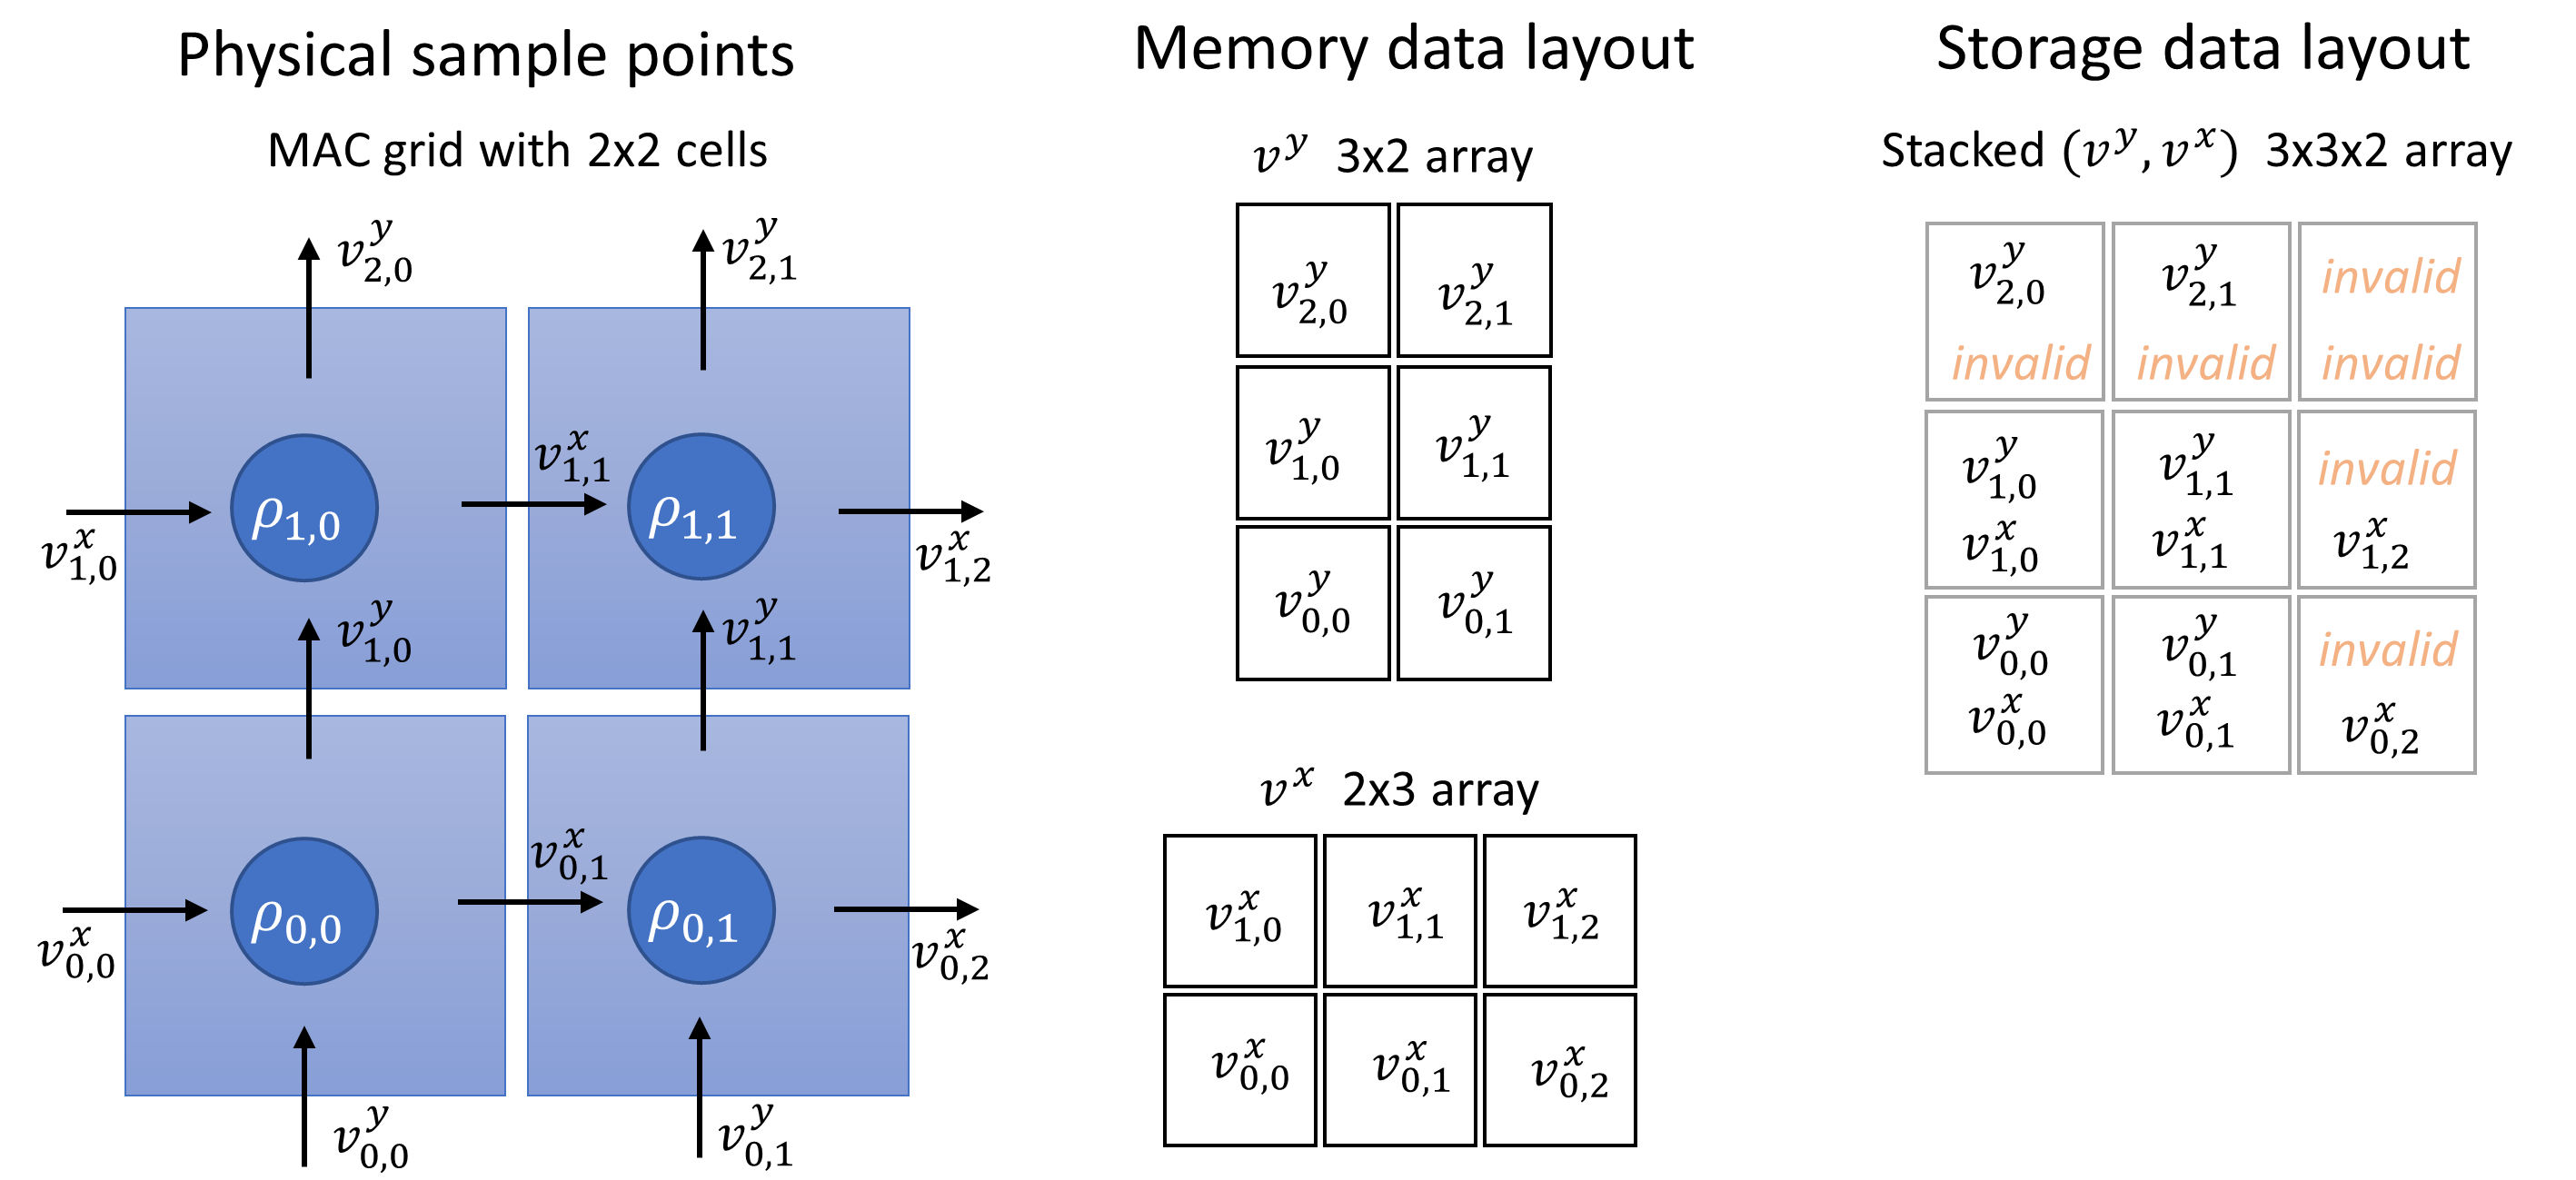
\includegraphics[width=\textwidth]{Staggered.png}
\caption{Staggered grid format \cite{staggeredform}}
\end{figure}

\subsection{Advection}
\begin{algorithm}\captionsetup{labelfont={sc,bf}, labelsep=newline}
	\caption{Incompressible fluid simulation algorithm}
\begin{algorithmic}
	\STATE {${\nabla}\cdot\vec{u} \gets 0$ (start with an initial velocity field $\vec{u}^{0}$ with the property)}
	\STATE {choose a time step $\Delta t$}
	\FOR {$n \gets 0, 1, 2, ...$}
	\STATE $\vec{u}^{A} \gets advect(\vec{u}^{n}, \vec{u}^{n}, \Delta t)$
	\STATE add the extra force $\vec{u}^{B} \gets \vec{u}^{A} + \Delta t\vec{g}$
	\STATE $\vec{u}^{n+1} \gets make\_incompressible(\Delta t, \vec{u}^{B})$
	\ENDFOR
\end{algorithmic}
\end{algorithm}

With the knowledge base of the NS-equation and grid structures we now need the advection algorithm to run the simulation. We adopt the semi-lagrangian advection algorithm. In the lagrangian point of view, if we want to compute the grid value of the n+1 time step of grid position $\vec{x_G}$, we should figure out which particle actually flows to the grid $\vec{x_G}$ from time step n. If we name the grid position of the particle as $\vec{x_P}$, then the new particle at time step n+1 in $\vec{x_G}$ should have the same physical property as the particle at time step n in $\vec{x_P}$

\begin{figure}[h]
\centering
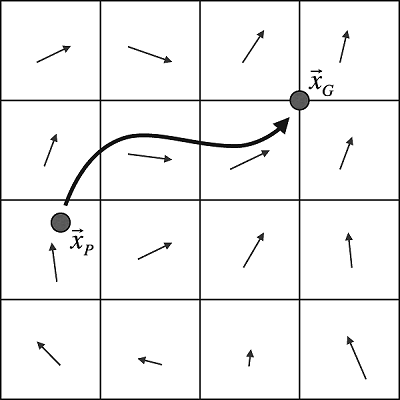
\includegraphics[scale=0.5]{advection.png}
\caption{advection\cite{semi}}
\end{figure}

we first use the euler equation to calculate the $\vec{x_P}$ as a step before of $\vec{x_G}$
\begin{equation}
\vec x_P=\vec x_G-\Delta t\frac{d\vec x_G}{dt}
\end{equation}

because $\frac{d\vec x}{dt}=\vec u(\vec x)$ we have

\begin{equation}
\vec x_P=\vec x_G-\Delta t\vec u(\vec x_G)
\end{equation}
where $\vec u(\vec x_G)$ denotes the velocity sampled at the position $x_G$, with the advection we can update the velocity, pressure and density of the whole vector field.

with all the knowledge above, we can formulate a sequence to conduct the basic fluid simulation.(see Algorithm 1)


\section{Deep learning tasks}
In this section, we introduce several fluid simulation related tasks which we focus on in this thesis.
\subsection{Autoencoder}
The Autoencoder model has a bottle neck shape, which aims to produce the same output as the input. Once trained, the Autoencoder model can be separated into two parts, namely the encoder and the decoder, which can compress the image with the encoder and later decompress the image with the decoder to its former shape.
\subsection{Super-resolution}
With the super-resolution model, we can upscale the low-resolution images to high-resolution images. The model is able to up-sample fluid simulation images if we feed similar data to train the model. In this paper, we apply the super-resolution model at the end of the Solver in the Loop model in order to boost the fluid simulation. Meanwhile, the simulation still obtain a similar output to the traditional simulation.
\subsection{Solver in the Loop}
When we want to perform our fluid simulation on a lower-resolution domain to decrease the time cost, we always suffer from the numerical error comparing to the simulation running on the higher-resolution domain. It is reasonable because with the same initial state, the vector field on the higher domain has richer information than the one sampled in the lower domain. \citeauthor{um2020sol} developed a mechanisim to learn the difference between the 2 different domains to reduce the numerical error.  We use the simulation from a high-resolution domain as the ground truth and make another same simulation with a lower resolution to approach our reference.  




\chapter{Related Work}
\paragraph{Perceptual losses related}The idea of jumping out of the traditional metrics based on $L^p$ norm has firstly begun by \cite{wang2004}, who developed the structure similarity index. Yet it was still not a perceptual loss and can not extract any deep features of the images. The situation has been improved by the discovery of CNN. CNNs are able to extract a lot of deep features, structures and patterns from the image datasets (for example in 2014 \cite{simonyan2014very} has proposed the VGG structure which achieved 92.7\% top-5 test accuracy in ImageNet), therefore more and more  works tend to use perceptual loss to train their models\cite{amirshahi2016, berardino2017, bosse2016, kang2014, kim2017}. In 2016 \cite{johnson2016perceptual} used intermediate layer comparison from the trained VGG-16 network to evaluate their model for both super-resolution task and style-transfer task.  in 2018 \cite{zhang2018perceptual} developed a new metric used for quality assessment as well as perceptual loss function. In 2020 \cite{kohl2020learning} proposed a new perceptual metric focusing on the numerical evaluation data.
\paragraph{Fluid simulation related}The PDE model of adopting NS-equation in fluid simulation has firstly been brought up by \cite{doi:10.1063/1.1761178} in 1965. Then PDE models with machine learning started to be popular \cite{crutchfield1987equations,kevrekidis2003equation,brunton2016discovering}. More recently deep learning started to play an important role in fluid dynamics\cite{kutz2017}. In 2019, \citeauthor{barsinai2019data} successfully integrate deep learning method into advection-diffusion problems to infer stencils. With the development of Phiflow \cite{holl2020learning}, beside performing physical simulations, we are able to integrate different deep learning backends (Tensorflow and Pytorch), so that we can track the gradient of the vectors that are stored in different grid formats. With the help of Phiflow, \cite{um2020sol} used Phiflow based deep learning methods to reduce the numerical error when performing fluid simulations. In 2020 \citeauthor{kim2020lagrangian} developed a neural style transfer approach from images to 3D fluids formulated in a Lagrangian viewpoint. Instead of using grid-based structure, \citeauthor{kim2020lagrangian} used particles for style transfer, which significantly reduce the training time.



%------- chapter 2 -------

\chapter{Metrics and Perceptual Losses}
Perceptual loss functions are used when comparing two images. They are different from traditional loss functions. For instance, MSE or MAE only compute the low level pixel differences. Perceptual losses on the other hand, are normally forward networks trained for specific tasks. For example, VGG-16 network was trained for massive image classification, and LSiM was trained on smoke and fluid simulations. When adopting those perceptual loss networks, we can either compute the MSE loss between the intermediate layers of the trained network, or pass through the trained perceptual loss network depending on the original goal of the chosen network. These perceptual loss networks try to retrieve the high level differences between the images, hence will usually have a better training performance than the traditional loss functions.

In this thesis we mainly focus on comparing the performance between traditional loss function MSE and perceptual loss functions LSiM, VGG-16 and Lpips. In this chapter we will cover these loss functions that we adopted in this paper and briefly explain their characteristics and their drawbacks. More precise integration and results will be covered in the Chapter 5. 

\section{Mean Square Error}

MSE is one of the most widely used loss functions.
\begin{equation}
{MSE}=\frac{1}{n}\sum_{i=1}^n(Y_i-\hat{Y_i})^2
\end{equation}
Where ${Y}$ is the reference tensor and $\hat{Y}$ is the predicted tensor based on the trainable parameters of the model. The optimal case is that the predicted tensor $\hat{Y}$ is exactly the same as the reference tensor ${Y}$. We can see that the core idea for the MSE is very general so that this loss function can be applied almost for any models, however the MSE loss function is not suitable for some image related tasks. If the two inputs of the MSE loss function is merely a image with its core content shifted by some pixels, the MSE will produce a very high value, which is not representitive, in another word, the MSE does not have shift or rotate invariance. 

Besides, MSE computes the square error of the two tensors, which means that MSE is also prone to the outliers, beacause when it has a very large outlier in the tensor, the result of MSE loss function will be strongly influenced, so in most image construction cases, in order to achieve a lower square error, the output will be a relative blur one compared with the original. Because a sharper image means that the difference between pixel values is huge, which will result in the high square error. On contrary, a blur image means that the pixel values have smaller distance, which will more likely achieve a lower square error. When MSE being adopted, the loss function would rather have a blur area than having a sharp outlier.
\begin{figure}
\centering
\begin{subfigure}{0.4\textwidth}
  \centering
  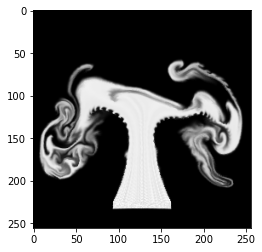
\includegraphics[scale=0.5]{MSEref.png}
  \caption{ref}
\end{subfigure}
\begin{subfigure}{0.4\textwidth}
  \centering
  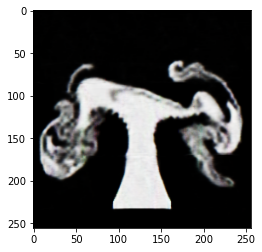
\includegraphics[scale=0.5]{MSEblur.png}
  \caption{MSE output}
\end{subfigure}
\end{figure}
 
\section{LSiM}

LSiM \cite{kohl2020learning} is a neural network-based approach that computes a stable and generalizing metric. Due to the unreliability of the MSE loss in numerical simulation tasks, LSiM has been established. It aims to demonstrate the performance of CNN-based evaluations on numerical simulation tasks. The data used to train LSiM are generated with known partial differential equations (PDEs). 

With figure \ref{lsimcompare}, we can tell that the $L^2$ loss function consider plume (b) a closer image to the reference, while the fact is that plume (a) has a smaller distance to the reference image, which is exactly predicted by the LSiM. Notice that the so called ground truth in this case is determined by shifting some initial parameters of the simulation. If the initial parameters are more closer to those of the reference simulation, then the GT distance will be respectively smaller.

\begin{figure}
\centering
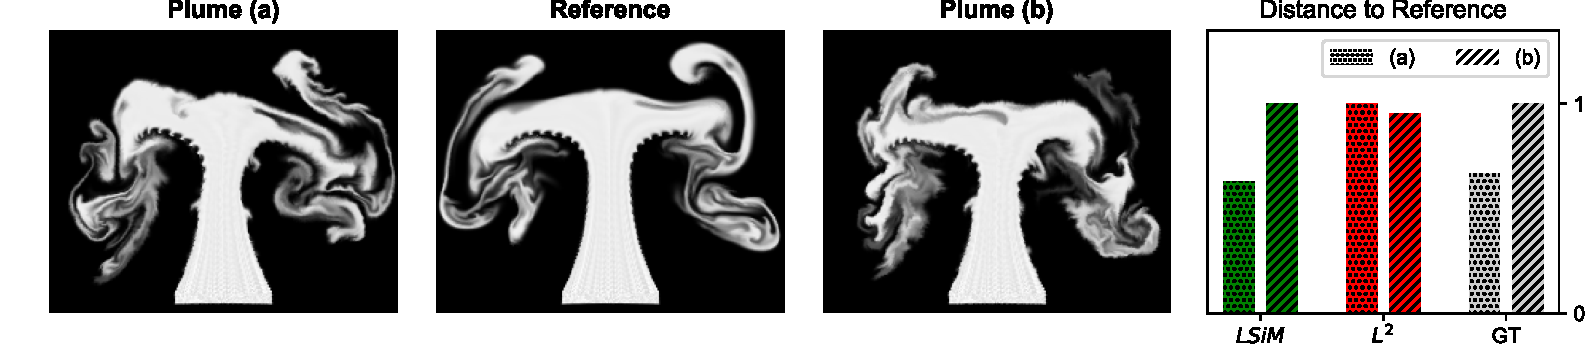
\includegraphics[width=1.0\textwidth]{Plumes.pdf}
\caption{The loss computed between two different plume images and the reference with LSiM and $L^2$ metrics. While the GT is the ground truth distance determined by the distance of the initial parameters in the data generation. }
\label{lsimcompare}
\end{figure}
The LSiM itself is also a CNN-based metric, see figure \ref{lsim}. The input of the network must be two batches of images with 3 channels
\begin{figure}
\centering
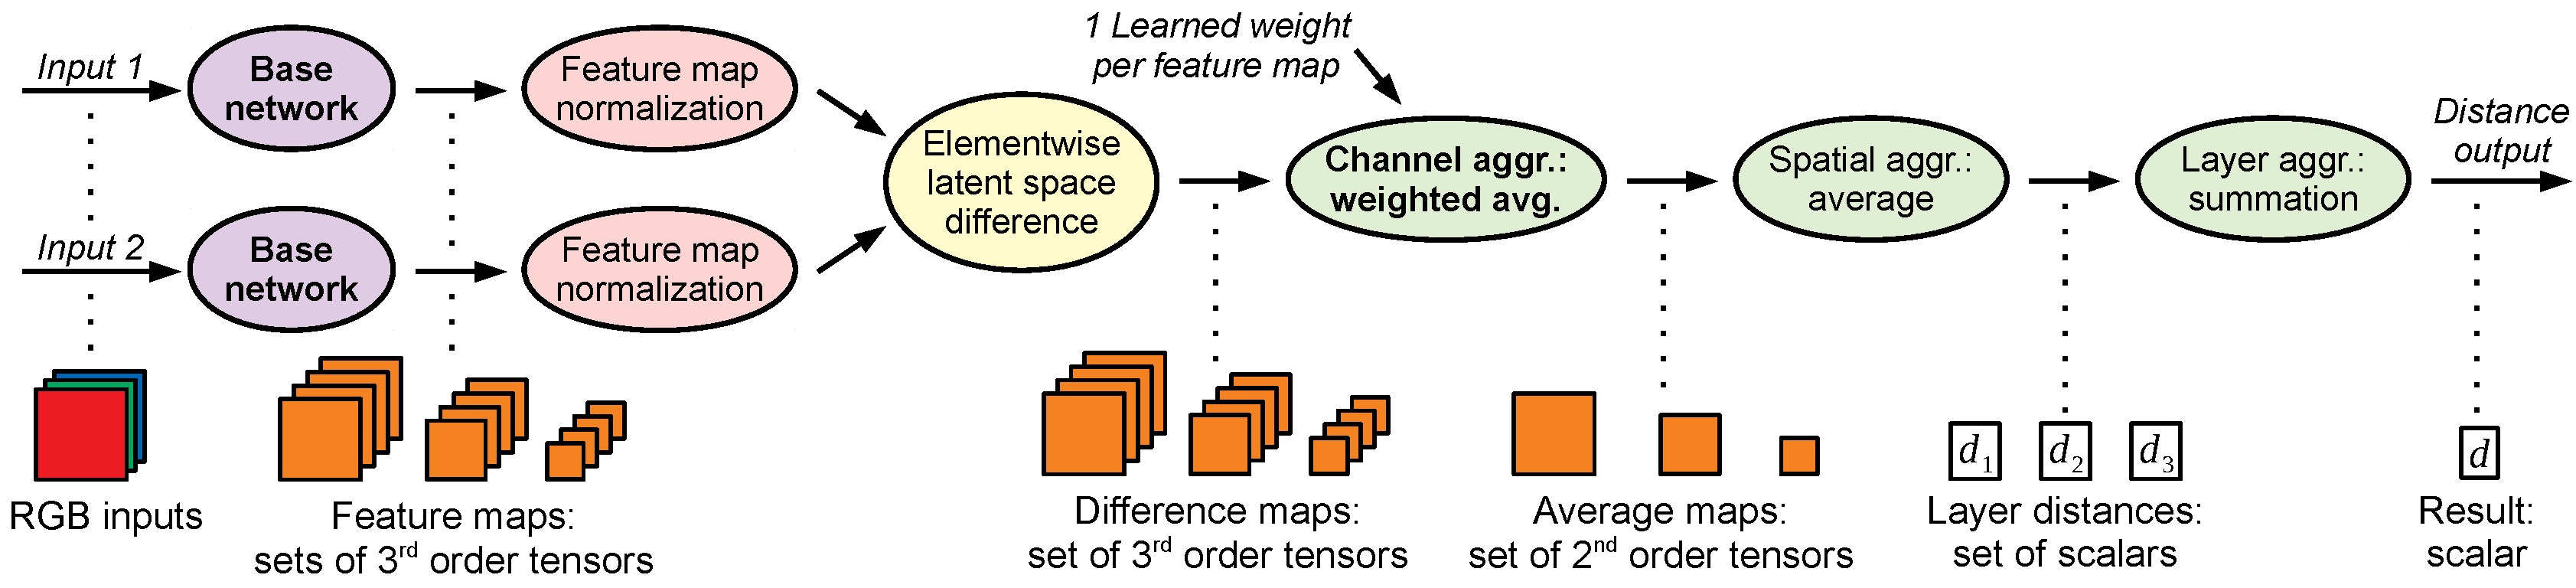
\includegraphics[width=1.0\textwidth]{DistanceComputation.pdf}
\caption{The Network structure of LSiM}
\label{lsim}
\end{figure}

As a metric, it also holds the metric properties $\forall \vx,\vy,\vz \in \sI$:
\begin{align}
    m(\vx,\vy) \; &\geq \; 0                && \text{non-negativity} \label{eq: NonNeg}\\
    m(\vx,\vy) \; &= \; m(\vy,\vx)              && \text{symmetry} \label{eq: Sym}\\
    m(\vx,\vy) \; &\leq \; m(\vx,\vz) + m(\vz,\vy)  && \text{triangle ineq.} \label{eq: TriIneq}\\
    m(\vx,\vy) \; &= 0 \; \iff \; \vx = \vy     && \text{identity of indisc.} \label{eq: IoI}
\end{align}
In terms of application, LSiM is already itself a perceptual loss network.  According to \citeauthor{kohl2020learning}, we need to form a dictionary consisting of two image inputs. When we feed the dictionary into the LSiM network, the output will be the loss value.
\section{VGG-16 loss network}

VGG-16\cite{simonyan2014very} is originally a CNN-based network trained for image classification problems. The author proposed 6 versions of VGG networks with different numbers of CNN layers but applied 3 fully connected layers for all of them at the end to realize the classification functionality. We adopted in the paper only the pretrained VGG-16 network(see figure \ref{vgg-16}) and apply it as a perceptual loss function.This pretrained model achieves 92.7\% top-5 test accuracy in ILSVRC-2014, which is a challenge based on a dataset of over 14 million images belonging to 1000 classes. Although the network was not originally trained for computing the distance, we can still use transfer learning to use it as a perceptual loss. In the paper\cite{johnson2016perceptual}, they chose to extract the third intermediate layer outputs and compute the MSE loss between them to realize the perceptual loss functionality(shown in figure \ref{vgg-16-perceptual})
\begin{figure}
\centering
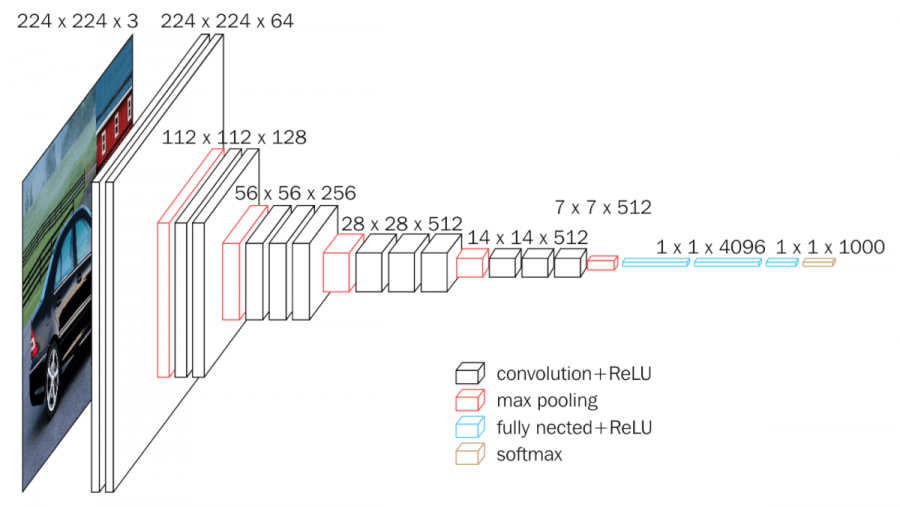
\includegraphics[width=1.0\textwidth]{vgg16.png}
\caption{The network structure of VGG-16}
\label{vgg-16}
\end{figure}
\begin{figure}
\centering
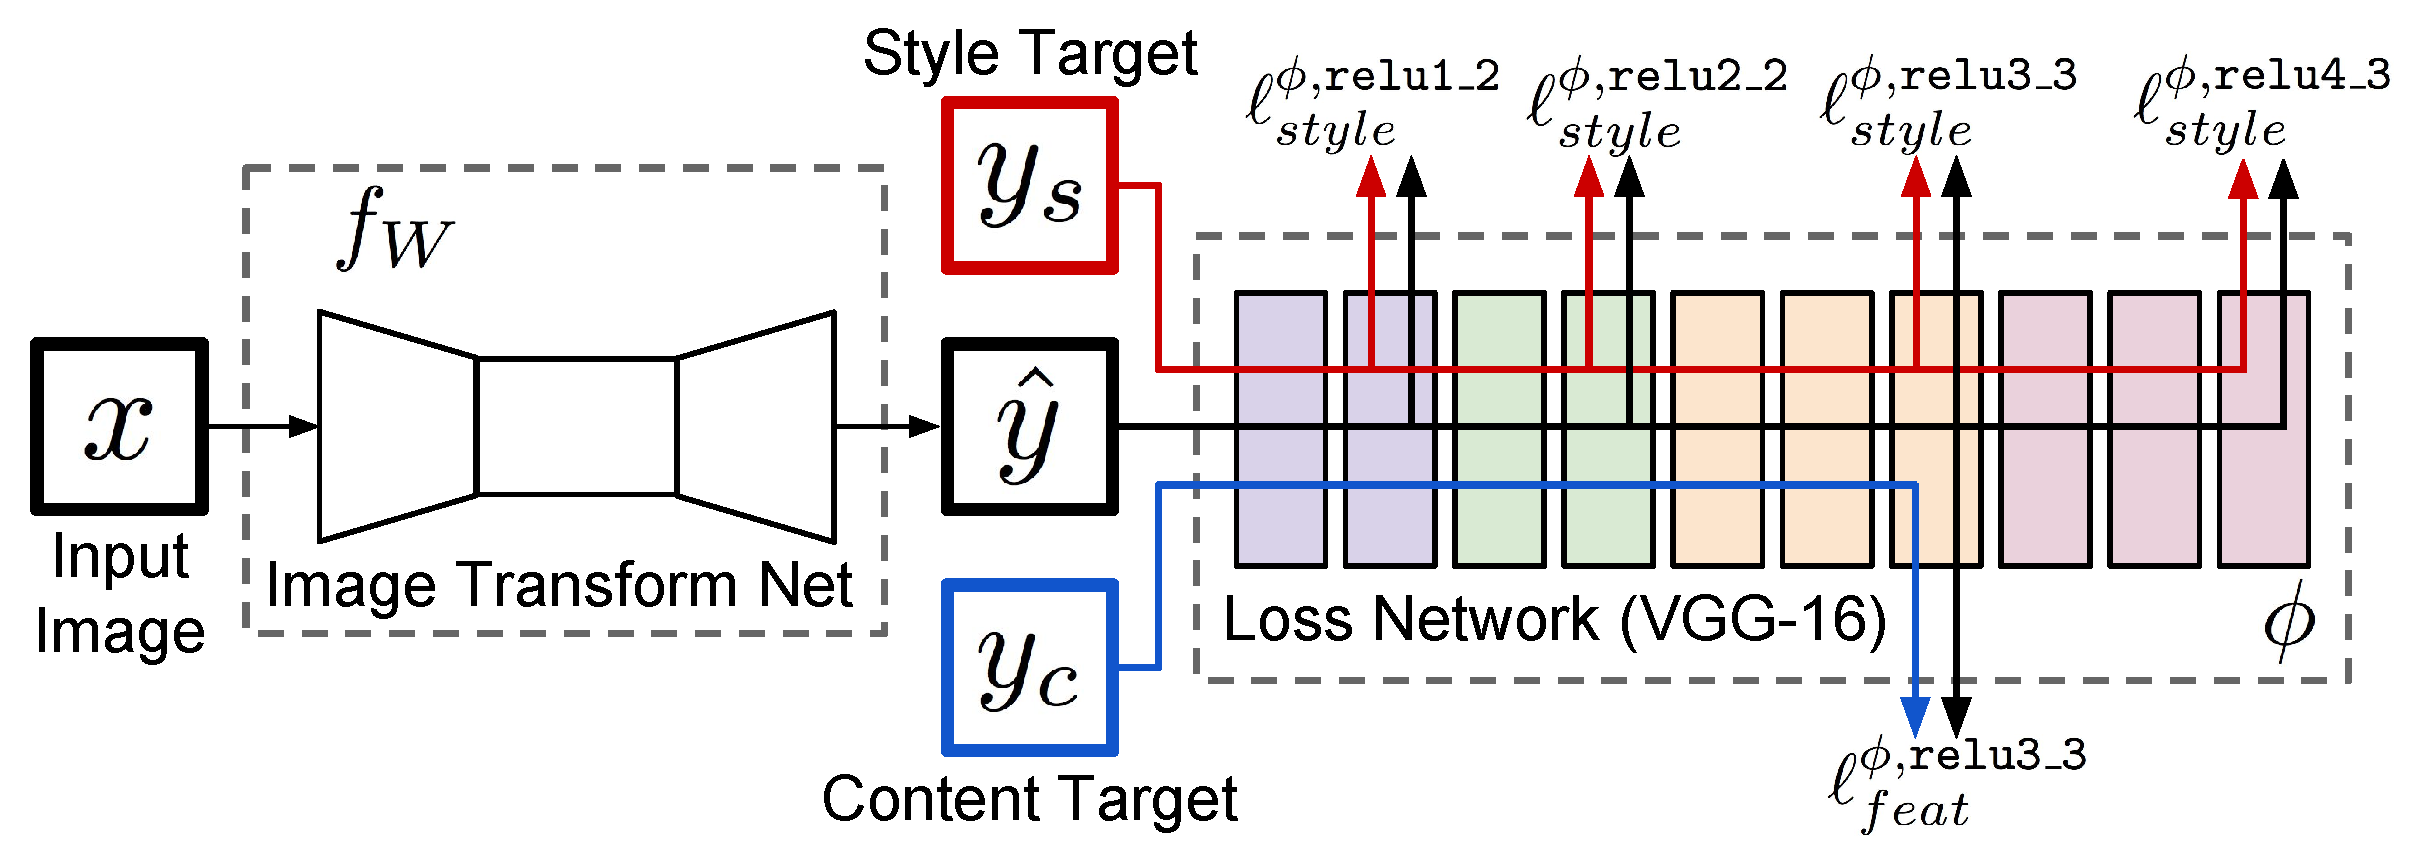
\includegraphics[width=1.0\textwidth]{SystemFigure.pdf}
\caption{How to extract the intermediate layer outputs of pretrained VGG-16 network to compute the loss.\cite{johnson2016perceptual}}
\label{vgg-16-perceptual}
\end{figure}
Apart from that we have also tested extracting the first, second or the fourth intermediate layers to calculate the MSE loss in order to compare the performance with the current method. We found out that computing MSE between the third one has the best performance in our training task.

\section{Lpips}
Lpips as in Learned Perceptual Image Patch Similarity\cite{zhang2018perceptual} is also a trained network to compare the high level image features based on various distortions. According to the author, they adopted distortions like CNN-based distortions, super-resolution, frame interpolation and so on for the dataset. Based on that, they use several psychophysical similarity measurements on the dataset, trying to approach the human judgements to the images. For the network architecture, they evaluate the SqueezeNet, AlexNet, and VGG architectures. We can consider Lpips as a advanced version of VGG-16, because we do not only consider certain intermediate layer outputs, moreover we take advantage of more intermediate layer outputs and the perceptual judgement, which will be a more reliable than just computing their MSE difference. We in this project choose to use the AlexNet based Lpips.
\begin{figure}
\centering
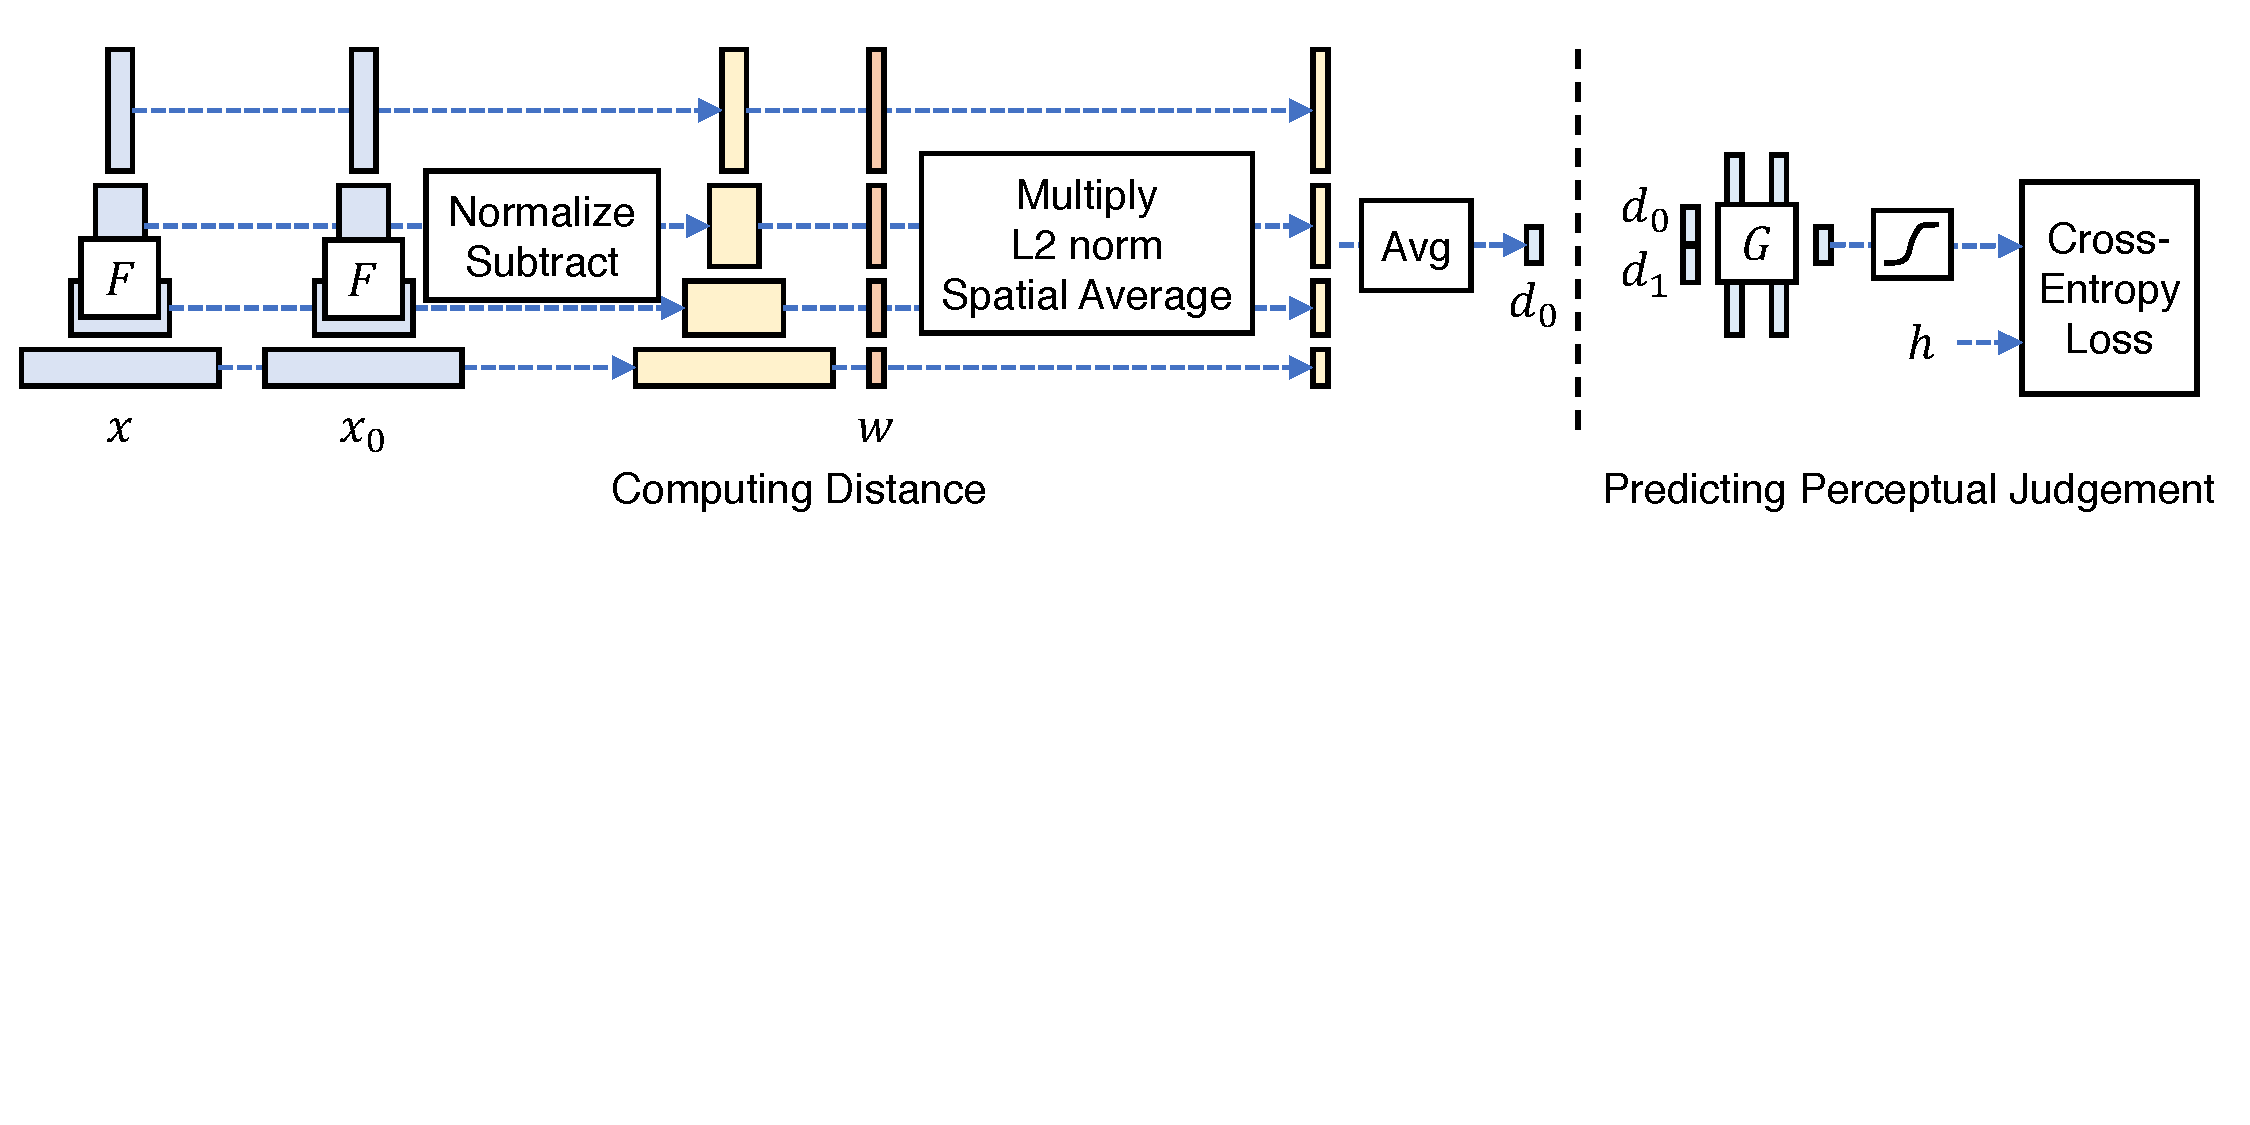
\includegraphics[width=1.0\textwidth]{network_lpips.pdf}
\caption{The Lpips training setup: The distance is computed between the ground truth patch $x$ and the distorted patch $x_0$ or $x_1$ based on the chosen network architecture. The perceptual distance is then trained on a small network $G$. The ground truth of the model outputs is the Psychophysical Similarity Measurement $h$ , and the training is based on the Cross Entropy Loss\cite{zhang2018perceptual}}
\end{figure}






%------- chapter 4 -------

\chapter{Datasets}
In this chapter we will cover the various datasets that we have adopted for training, validation and testing in the following three tasks.

\section{Autoencoder}
We set up the Autoencoder mainly to have a rough overview of the performance of the perceptual loss functions. Hence, we choose to use the numerical simulation data with the original size of 256*256, on which the LSiM model was trained. 

Autoencoder can be trained without supervision, because the training data is exactly the reference, so we do not need to do any modification to complete the training. However, in order to accelerate the training, we made 2 following modifications:
\begin{itemize}
\item since the numerical simulation data are mostly gray scale, which means we can sample them with one channel to boost our training and replicate the channel when certain loss functions demand their inputs in RGB channels. Such techniques can also be applied on any models with grayscale data, you can see more details about it in the Section 5.2.2.
\item in order to reduce the GPU usage, we downsample the 256*256 training data to the size of 128*128.

\end{itemize}


\section{Super-resolution}
The data we used in the super-resolution task came from various sources. We first used the training data of LSiM model, because these are all numerical simulation data including the velocity, density and pressure images, so we recon that LSiM can outperform the other metrics.
\begin{figure}
\centering
\begin{subfigure}{0.3\textwidth}
  \centering
  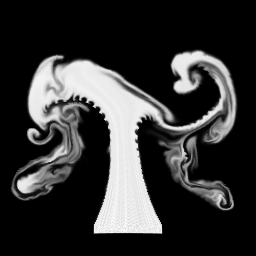
\includegraphics[scale=0.5]{density.png}
  \caption{density data}
\end{subfigure}
\begin{subfigure}{0.3\textwidth}
  \centering
  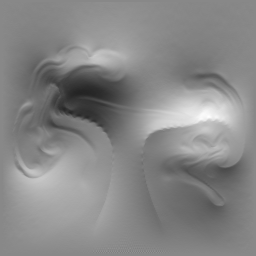
\includegraphics[scale=0.5]{velocity.png}
  \caption{velocity data}
\end{subfigure}
\begin{subfigure}{0.3\textwidth}
  \centering
  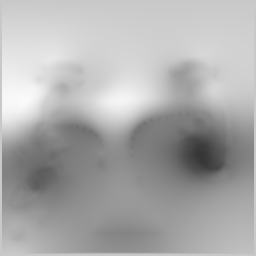
\includegraphics[scale=0.5]{pressure.png}
  \caption{pressure data}
\end{subfigure}
\caption{Training set of LSiM model}
\end{figure}

We also want to test the performance of combining Solver in the Loop and super-resolution together to compete against the time cost with performing the simulation purely on the higher domain. Therefore we also feed the training data of the Solver in the Loop to the super-resolution model, so that our model can learn to super sample the plume density images when we feed the corrected simulation images on the lower domain. In this way, we are able to abtain the plume images with the same resolution as the higher domain.Apart from that, we also test the our model performance on some random videos data which are not related to numerical simulations but still can be of some assistance to our model.

To create the data set, we form a dictionary for each image. We first downsample each training image $I_{high}$ to a lower resolution image $I_{downsampled}$(e.g. images of 256*256 to image of 64*64), then we resize the $I_{downsampled}$ to the same image size of the previous $I_{high}$, then we get a image $I_{low}$ with the same image size but a lower resolution as the $I_{high}$. In the training process we treat the $I_{low}$ as the input data of the model, $I_{high}$ as the groud truth to compute the loss with the model output.
\section{Solver in the Loop}
\subsection{Simulation tasks}
In the Solver in the Loop tasks, we have trained and tested out our model with 2 different fluid simulations, which are the 2-D karman flow and 2-D buoyancy driven flow. \citeauthor{um2020sol} has mainly trained their model on the karman flow, based on which we extend the model to a more complex simulation i.e. the buoyancy driven flow. 

For both simulation tasks, we have prepared two datasets with different resolutions in order to compare the performance of different loss functions on different resolutions. The two resolutions we chose for the karman flow are 128*64 and 64*64, and for buoyancy driven flow tasks we picked 64*64 and 128*128. As we want to reduce the numerical error for the model trained on a lower domain, for each resolution ratio we have to firstly generate a higher resolution dataset as the reference dataset. However, we can not compare two datasets with different resolutions. Therefore we have to down-sample the higher resolution training set to a lower one that matches our training domain. Afterwards, the down-sampled dataset with rich simulation details from higher domain is our actual reference set.

\begin{figure}
\centering
\begin{subfigure}{0.4\textwidth}
  \centering
  
\includegraphics[scale=0.5]{karmanflow.png}
  \caption{Karmanflow example}
\end{subfigure}
\begin{subfigure}{0.4\textwidth}
  \centering
  
\includegraphics[scale=0.5]{buoyancy.png}
  \caption{Buoyancy driven flow example}
\end{subfigure}
\caption{Two simulation examples for Solver in the Loop}
\end{figure}

\begin{figure}
\centering
\begin{subfigure}{0.4\textwidth}
  \centering
  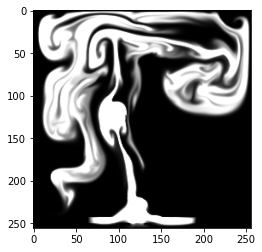
\includegraphics[scale=0.5]{buoyancy_high.png}
  \caption{Buoyancy driven flow image with 256*256}
\end{subfigure}
\begin{subfigure}{0.4\textwidth}
  \centering
  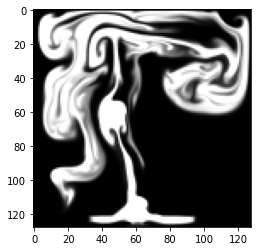
\includegraphics[scale=0.5]{buoyancy_ds.png}
  \caption{Downsampled buoyancy driven flow image with 128*128}
\end{subfigure}
\caption{Reference images generation and downsampling}
\end{figure}
\subsection{Phiflow setup}
The tool we used to perform the fluid simulation is Phiflow\cite{holl2020learning}. 

For the karmanflow generation, we define an open domain with the size of 200(height) * 100(width)\footnote{notice that domain size is not the same concept as the domain resolution. The domain size helps to locate the position of the inflow and obstacles of the simulation, while the resolution is used to define how percise we should sample our domain. Hence we could perform different resolution formats on the same domain size.} we set the inflow as a 5 * 50 rectangle at the top center, and the obstacle as a circle with radius 10 positioned in the very center of the upper half of the domain. The step size $\Delta t$ we chose here is 1.0. For each simulation we chose to generate 1500 frames for the karman flow.

For the buoyancy driven flow generation, we define a 200 * 200 closed domain and set the inflow as a 5 * 100 rectangle at the bottom center. We generate 250 frames for the high-resolution simulation and 150 for the low-resolution one. Why we only chose 250 steps and 150 steps for the buoyancy driven flow is because we defined a closed boundary for the buoyancy flow so the simulation after 250 steps are extremely complex, and we also set the timestep to 0.1 to slow down the simulation so we will not have a chaotic frame of plumes. Which helps to make our training easier.

For both tasks, we have a total of 8 simulations with their renolds numbers ranging from $1*10^5$ to $8*10^5$ as the training set. As for the test set we can alter the renolds number and the seed of the simulation to generate a sets of simulation frames that are overall similar but in details deviated from the used training set. 
\begin{figure}
	\centering
	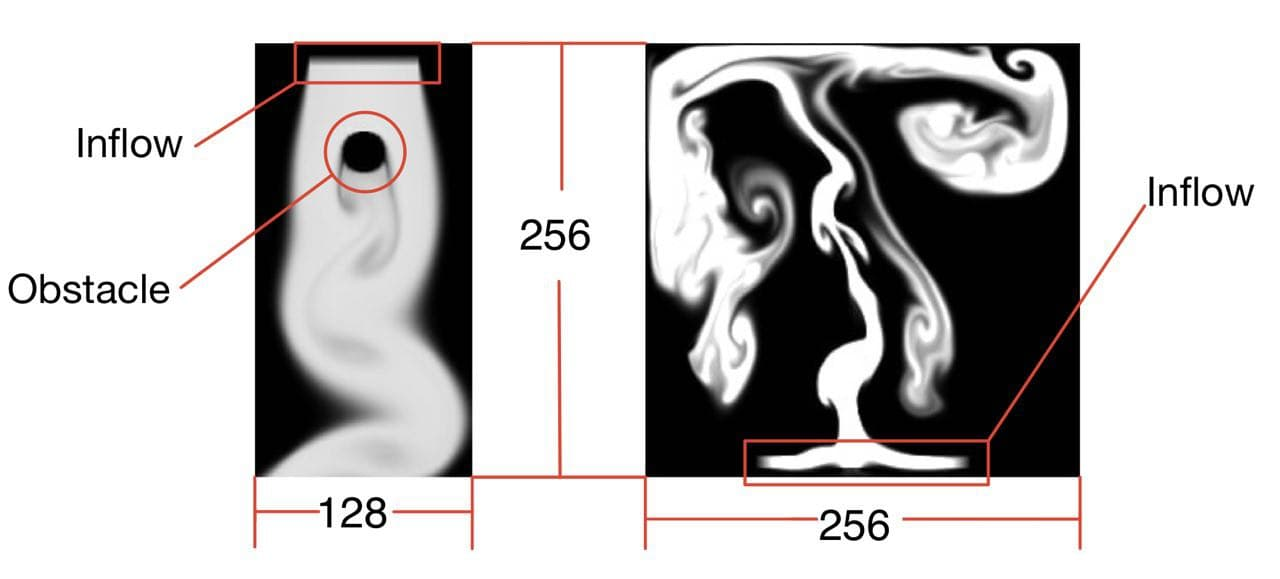
\includegraphics[width=1.0\textwidth]{domaindescription.jpg}
	\caption{Domain set up of karman flow and buoyancy driven flow}
\end{figure}






%------- chapter 5 -------

\chapter{Tasks and Experiments Setup}

\section{Autoencoder}
\subsection{Network}
We used a very simple bottle-neck like and fully convolutional neural network for the Autoencoder(see figure 5.1). Due to the gray scale images, the input and output channel size is set to 1. We apply two convolution layers followed by one max pooling layer and two upsample convolution layer. In order to keep the tensor value within a reasonable range, we add before the final output a 256*sigmoid layer to ensure that every output value should lie in between [0, 255]. However sigmoid should not be used in the intermediate layers, which will cause vanishing gradient problem, so we use ReLU as the activation function for the intermediate layer. The reason why we do not add a ReLU activation function before the sigmoid is because the ReLU only outputs positive values which wil results in that the sigmoid function will then only output values greater then 0.5, then we will lose half of the value range of the images which is not acceptable.
\subsection{Application of loss functions}
Before feeding the input image to the model and compute the loss function, we can still add on some modification to make our training eaiser. Since most of our data are smoke images or velocity fields, so they are in gray scale. In this case, we can modify our network in the way that the new input channel size and the output channel size are 1, because the gray scale images only have one channel. With this modification, our model does not need to learn to align all the three RGB channels to the same value, hence it will strongly reduce the training difficulty. However, in the process of applying the loss function, there will be the problem that many of the perceptual loss functions only accept RGB images that the input tensors should have three channels. In order to fix this, we choose to replicate the channel size to three with the same value, so the loss functions will regard our gray scale images as RGB images. In this way we keep the tensors in the training process as one-channel tensors however in the loss function computation process as three-channels tensors, which increase our model performance.

In order to compute the loss functions, we need to define the reference and the model output. Now we know our first input is the model output with replicated channels, and the reference input should be the $I_{high}$. The rest is to define the respective metrics. For MSE loss we can directly compute it between two tensors. For VGG-16 loss function, we can feed each tensor into the model and compute MSE loss between their third intermediate outputs. For LSiM we can form a dictionary of these two tensors and pass it to the forward function of the LSiM model. For Lpips we can directly use the pretrained model and feed the two tensors into the function.


\begin{figure}
  \centering
  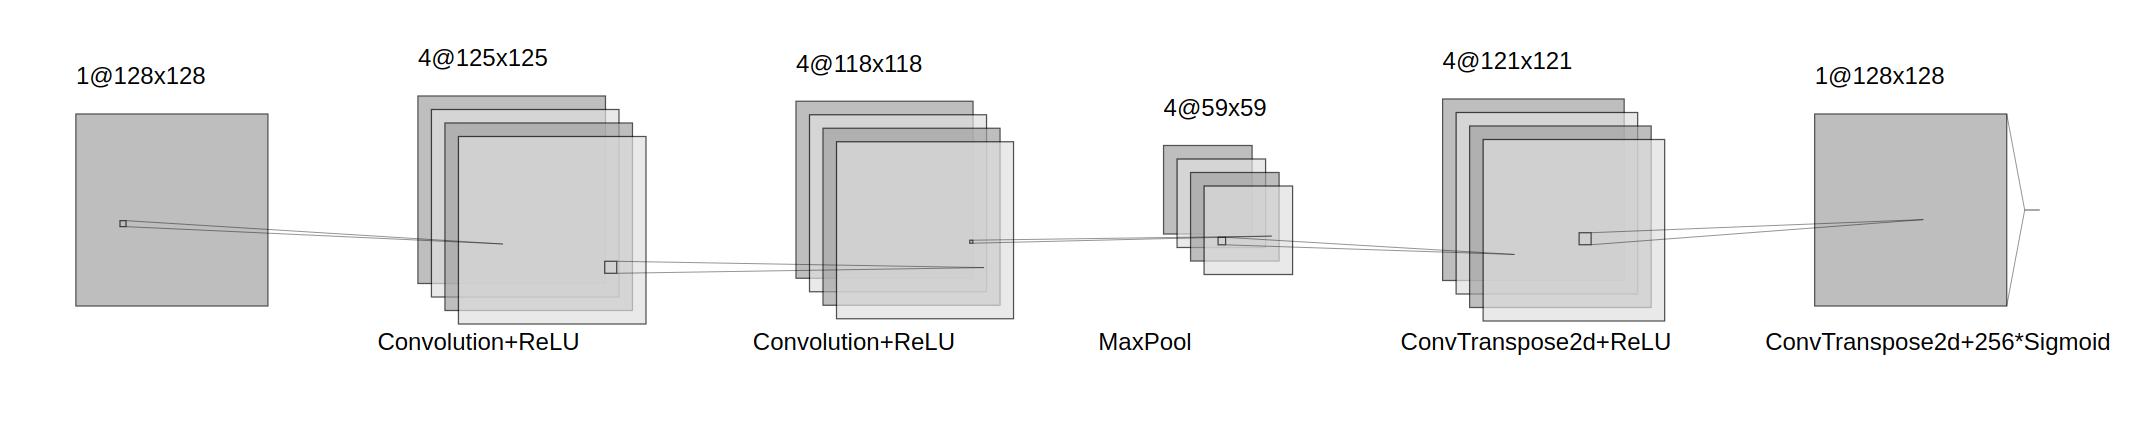
\includegraphics[width=\textwidth]{autoencoder.png}
  \caption{The structure of Autoencoder}
\end{figure}

\section{Super-resolution}
\begin{figure}
	\centering
	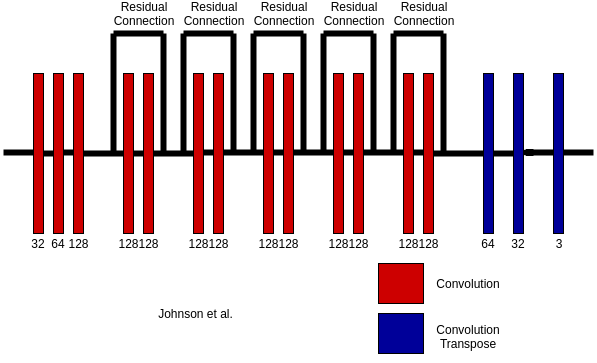
\includegraphics[scale=0.5]{ITN.png}
	\caption{The structure of ImageTranformationNetwork of \cite{johnson2016perceptual}}
\end{figure}
\subsection{Network}
\begin{figure}
	\centering
	\begin{subfigure}{0.49\textwidth}
		\centering
		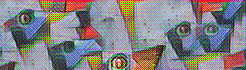
\includegraphics[scale=0.6]{style_artifacts.png}
		\caption{Using deconvolution. Heavy checkerboard artifacts.}
	\end{subfigure}
	\begin{subfigure}{0.49\textwidth}
		\centering
		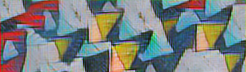
\includegraphics[scale=0.6]{style_clean.png}
		\caption{Using resize-convolution. No checkerboard artifacts.}
	\end{subfigure}
	\caption{The comparison between two upsample methods\cite{odena2016deconvolution}}
	\label{checkerboard}
\end{figure}

We adopt the same ImageTranformNetwork proposed by \citeauthor{johnson2016perceptual}, which is a fully convolutional network that has the same output tensor shape as the input. The network consists of three Convlayers, three UpsampleConvlayers and five residual blocks.\footnote{Notice that we do not use the deconvolutional layer in the UpsampleConvlayers as suggested in the paper\cite{odena2016deconvolution}, that deconvolutional layers will likely result into checkerboards artifacts due to the overlapping when doing the reverse convolution operations(see figure \ref{checkerboard}). So we prefer to fistly do the traditional upsampling either with Nearest-neighbor interpolation or with Bilinear interpolation then we apply the convlayer afterwards to obtain the expected upsampled size.}

Since the outputs of our model is RGB images, which means the tensor values lie in the range of [0, 255], so we apply at the end of the last upsampling layer a sigmoid function and then multiply 256. In such way, we can ensure that our output tensor value won't exceed the range. According to the model structure, the input tensor and the output tensor should share the same shape. So before we feed the low resolution data to the model, we need to first do the upsampling with some interpolation methods(we choose bilinear here) to resize our input images to the expected high resolution, then feed them to the model. 

\subsection{Application of loss functions}
The training process of super-resolution is very similar to that in the autoencoder task. The only different part is that we in the autoencoder use the same training data as the reference data, however in the super-resolution we use the downresoluted images as the training data. In terms of applying loss function, we also need to replicate the channels to suit the input shape of certain loss functions. For more details of how to deploy such modification, please turn to the Section 5.1.2


\section{Solver in the Loop}
After we have generated the training set and its down-sampled version, we can start the training. We will first cover the basics of the network and its training goal, then we will go into details of how to apply the loss function.
\subsection{Network}
The training network we used is called MarsMoon, which is the same network that \citeauthor{um2020sol} adopted in the his project(see figure \ref{marsmoon}) we can see that the number of channels for both input and output is 2. This is because the input is the staggered tensor of the velocity which has two directions one represents the y direction and the other represents the x direction. The output of the network is also a staggered tensor however it can not be directly addressed as the velocity but a correction of the velocity, which can be added to the velocity calculated on the lower domain, then the corrected velocity can be applied for the next simulation step. The reason why we do not train the output towards the velocity for the next simulation step is because we want to take advantage of the physical information stored in those tensors, if we should simply get the next velocity from passing the former velocity through the network, then we would not need to perform the physical simulation, which is very unstable. Thus, adding the trained correction to the physical simulation output of the former velocity would at least make sure that our simulation is performing on the right track. That means our consecutive steps of the simulation are based on valid physical simulation, which can not be ensured by purely passing through the neural network.
\begin{figure}
\centering
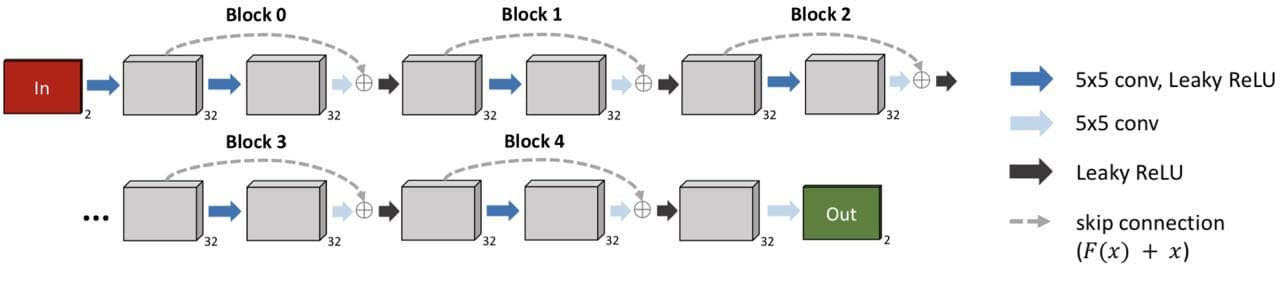
\includegraphics[width=1.0\textwidth]{marsmoon.jpg}
\caption{The network architecture\cite{um2020sol}}
\label{marsmoon}
\end{figure}

\begin{figure}
\centering
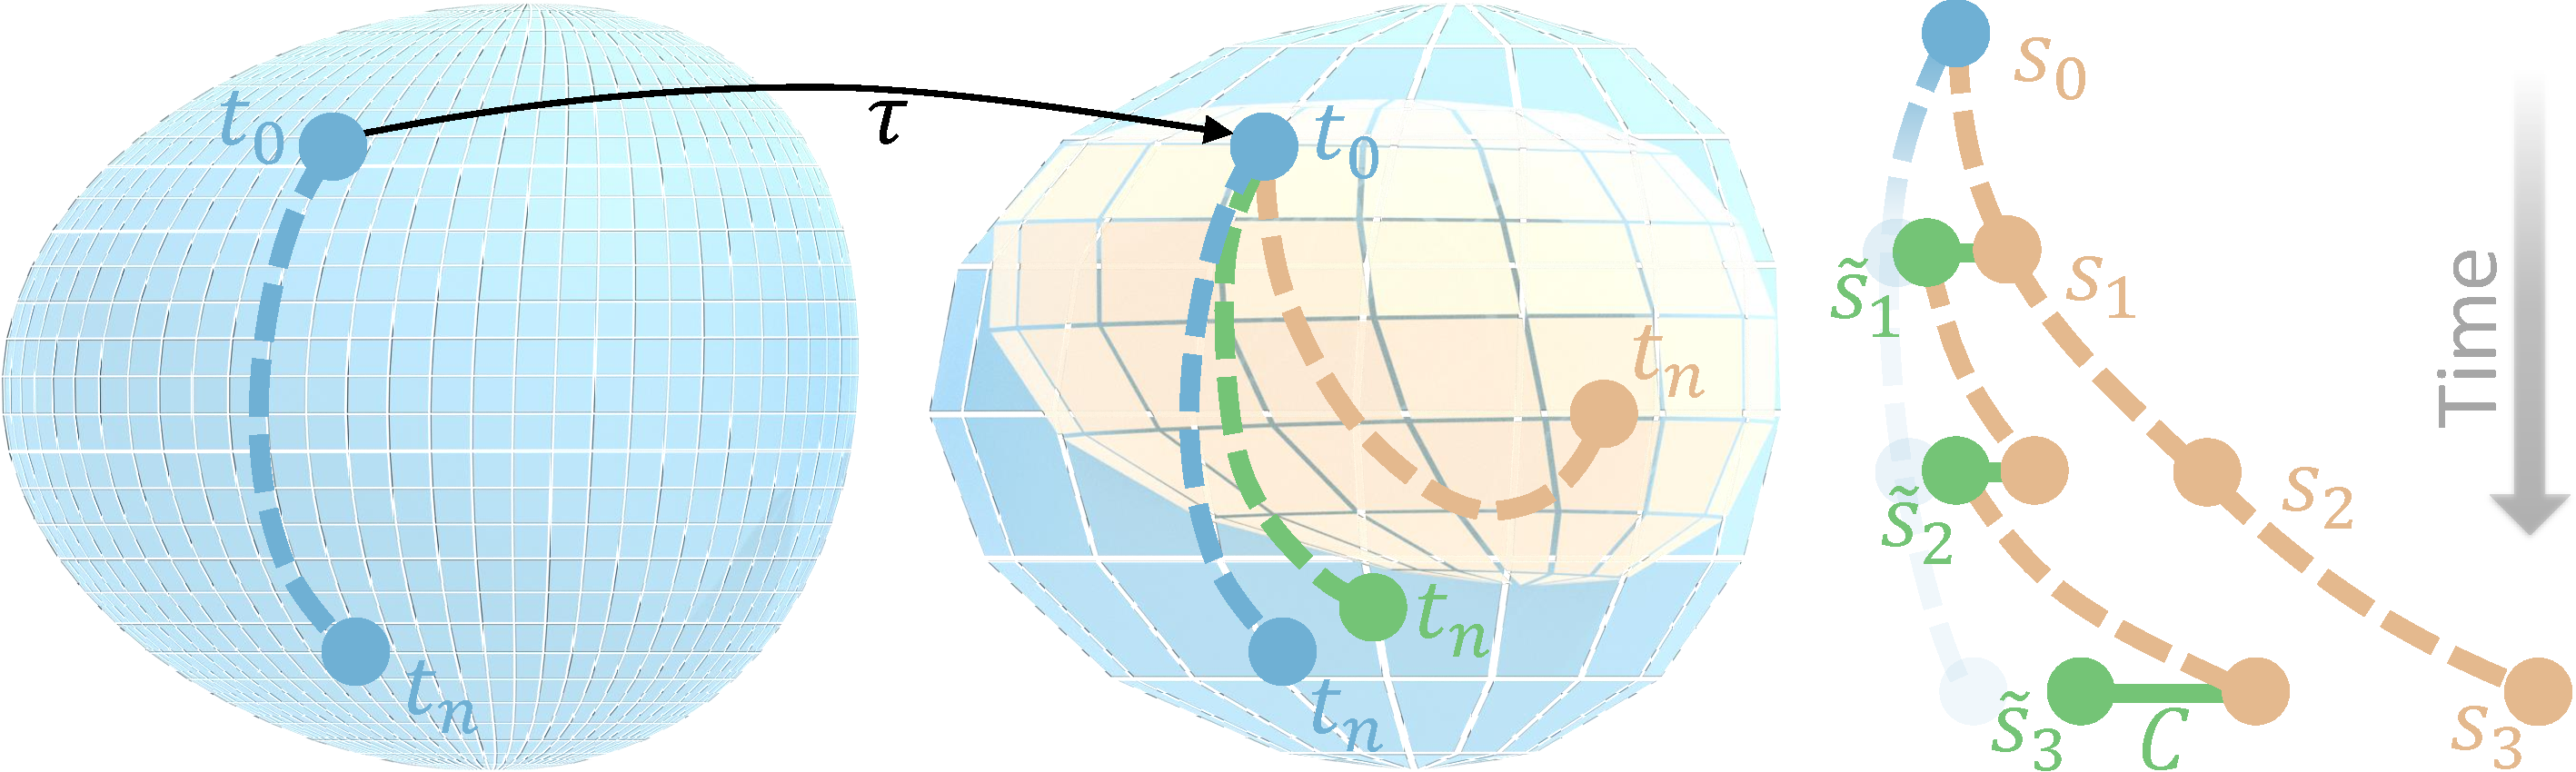
\includegraphics[width=1.0\textwidth]{Manifolds.pdf}
\caption{The training goal is to obtain the suitable correction, with which the simulation on the lower domain can reduce the numerical error. The brown one represents the source simulation of the lower domain without any corrections, the blue one represents the simulation on the higher domain which is our target, the green one is the brown one plus the trained correction, which aims to approach the blue one\cite{um2020sol}}
\end{figure}
\subsection{Training Set}
In karman flow simulation, we choose not to use the whole training set to train our model, because the first 1000 steps of the low-resolution karman flow have not deviated too much from the high resolution karman flow. So we only try to train the last 500 steps of the total 1500 steps to accelerate the training. We at the beginning trained the lower domain karman flow with the domain resolution of 64*32, but we found out that the 64*32 image for LSiM model is too small. So we decided to alter the domain to the resolution of 64*64, correspondingly the training set also need to be regenerated on the domain of 128*128. However the size of the plume remains unchanged, we only pad the domain such that they can be applied to LSiM loss function.(see figure \ref{pad})
\begin{figure}
\centering
\begin{subfigure}{0.4\textwidth}
  \centering
  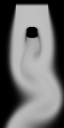
\includegraphics[scale=1]{nonpad_karmanflow.png}
  \caption{original simulation}
\end{subfigure}
\begin{subfigure}{0.4\textwidth}
  \centering
  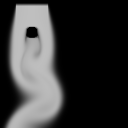
\includegraphics[scale=1]{pad_karmanflow.png}
  \caption{padded simulation}
\end{subfigure}
\caption{Padding plume images to match the input size of LSiM model. However, with the same parameters, there are still some differences between the padded and original karman flow simulation due to the domain size difference.}
\label{pad}
\end{figure}
For the buoyancy driven flow simulation, it only consists of 250 steps and each step has rich numerical information, so we regard the whole simulation as the training set. Besides, since the buoyancy simulation on the lower domain already has the shape of 64*64 we don't need to add extra padding to suit the LSiM model.


\subsection{Application of loss functions}
In order to compute the loss we have to define the 2 inputs of our loss functions. We know our model output is the correction, however it is unreasonable to directly compare the correction with the reference simulation. So the two inputs of the loss functions should be 
\begin{itemize}
\item $V$: The sum of the velocity tensor on the lower-domain simulation and the trained correction .

\item $\hat{V}$: The down-sampled velocity tensor from the higher-domain simulation(reference).
\end{itemize}


For the MSE loss, which is originally used by \citeauthor{um2020sol}, we can simply calculate their pixel wise square difference and compute their mean. This traditional loss function does not rely on the structure of the tensor as long as they share the same shape. So the MSE loss between two staggered tensors can be easily computed. However the perceptual loss function has some demands on our tensor shape due to its CNN structure. For example, LSiM requires that the input tensor should consist of 3 channels to represent the RGB channels, while the size of the input tensor should be large enough to pass through several conv-layers. In our case, the output of the model is a staggered tensor with 2 channels which respectively represent x and y directions. Our solution is, that we compute the loss over each direction separately and sum them up. We firstly both extract the x direction tensor $V_x$ and y direction tensor $V_y$ from our model output $V$, then we also extract the x direction tensor $\hat{V_x}$ and y direction tensor $\hat{V_y}$ from the reference velocity tensor $\hat{V}$. Our final loss function representation looks like:
\begin{equation}
 Loss(V, \hat{V}) = F(V_x, \hat{V_x}) + F(V_y, \hat{V_y})
\end{equation}
where F is the respective perceptual loss function. In this way, we are able to treat the velocity tensor on each direction as an image(or triplicate the channel to RGB image) and compare them with their ground truth.  






%------- chapter 5 -------

\chapter{Results and Analysis}

\section{Comparison}
\subsection{Autoencoder}

\begin{figure}
	\centering
	\begin{subfigure}{0.19\textwidth}
		\centering
		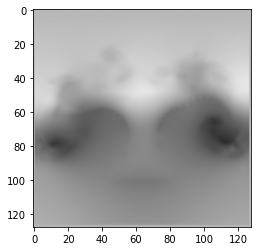
\includegraphics[scale=0.29]{autoencoder/ref1.png}
		\caption{$Reference$}
	\end{subfigure}
	\begin{subfigure}{0.19\textwidth}
		\centering
		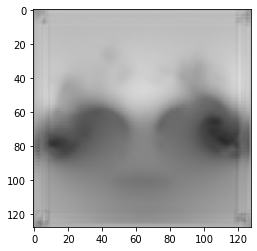
\includegraphics[scale=0.29]{autoencoder/mse1.png}
		\caption{$MSE$}
	\end{subfigure}
	\begin{subfigure}{0.19\textwidth}
		\centering
		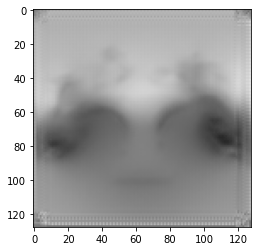
\includegraphics[scale=0.29]{autoencoder/lsim1.png}
		\caption{$LSiM$}
	\end{subfigure}
	\begin{subfigure}{0.19\textwidth}
		\centering
		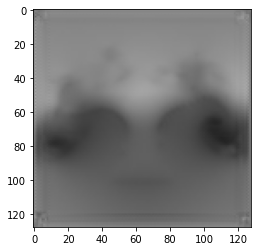
\includegraphics[scale=0.29]{autoencoder/lpips1.png}
		\caption{$Lpips$}
	\end{subfigure}
	\begin{subfigure}{0.19\textwidth}
		\centering
		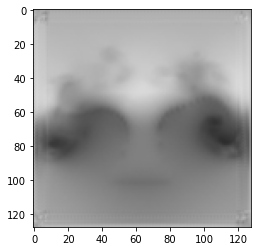
\includegraphics[scale=0.29]{autoencoder/vgg1.png}
		\caption{$VGG-16$}
	\end{subfigure}
	\caption{Pressure images reconstructions of autoencoder task}
	\label{autoencoder pressure outputs}
\end{figure}


\begin{figure}
	\centering
	\begin{subfigure}{0.19\textwidth}
		\centering
		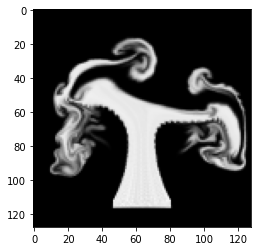
\includegraphics[scale=0.29]{autoencoder/ref2.png}
		\caption{$Reference$}
	\end{subfigure}
	\begin{subfigure}{0.19\textwidth}
		\centering
		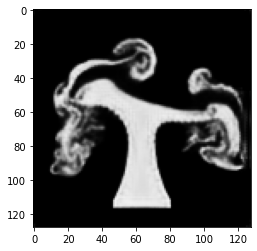
\includegraphics[scale=0.29]{autoencoder/mse2.png}
		\caption{$MSE$}
	\end{subfigure}
	\begin{subfigure}{0.19\textwidth}
		\centering
		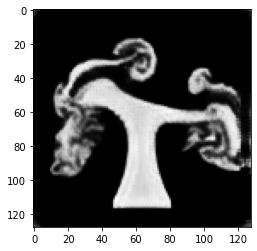
\includegraphics[scale=0.29]{autoencoder/lsim2.png}
		\caption{$LSiM$}
	\end{subfigure}
	\begin{subfigure}{0.19\textwidth}
		\centering
		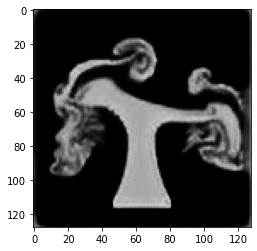
\includegraphics[scale=0.29]{autoencoder/lpips2.png}
		\caption{$Lpips$}
	\end{subfigure}
	\begin{subfigure}{0.19\textwidth}
		\centering
		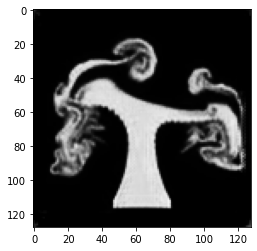
\includegraphics[scale=0.29]{autoencoder/vgg2.png}
		\caption{$VGG-16$}
	\end{subfigure}
	\caption{Density images reconstructions of autoencoder task}
	\label{autoencoder density outputs}
\end{figure}
 \begin{figure}
	\centering
	\begin{subfigure}{0.32\textwidth}
		\centering
		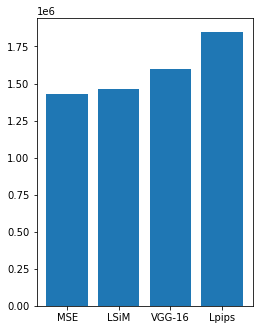
\includegraphics[scale=0.5]{autoencoder/l2eval.png}
		\caption{L2 evaluation}
	\end{subfigure}
	\begin{subfigure}{0.32\textwidth}
		\centering
		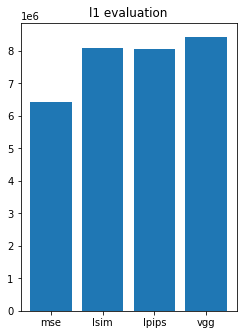
\includegraphics[scale=0.5]{autoencoder/l1eval.png}
		\caption{L1 evaluation}
	\end{subfigure}
	\begin{subfigure}{0.32\textwidth}
		\centering
		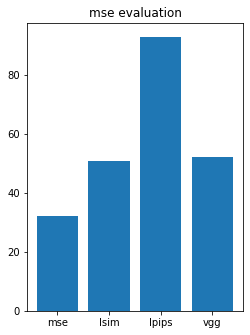
\includegraphics[scale=0.5]{autoencoder/mseeval.png}
		\caption{MSE evaluation}
	\end{subfigure}
	\begin{subfigure}{0.32\textwidth}
		\centering
		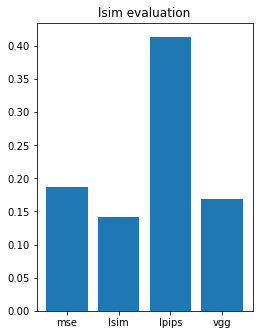
\includegraphics[scale=0.5]{autoencoder/lsimeval.png}
		\caption{LSiM evaluation}
	\end{subfigure}
	\begin{subfigure}{0.32\textwidth}
		\centering
		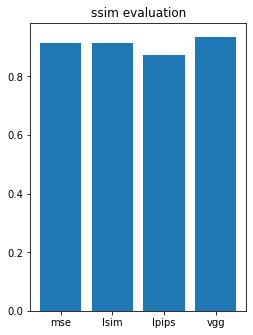
\includegraphics[scale=0.5]{autoencoder/ssimeval.png}
		\caption{SSIM evaluation}
	\end{subfigure}
	\begin{subfigure}{0.32\textwidth}
		\centering
		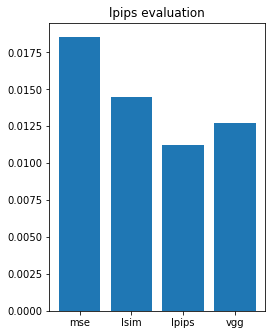
\includegraphics[scale=0.5]{autoencoder/lpipseval.png}
		\caption{Lpips evaluation}
	\end{subfigure}
	\caption{Numerical evaluation of each metric on the testset of autoencoder task}
	\label{autoencoder numeval}
\end{figure}
We train the autoencoder model on density, pressure and velocity data of smokes, here are some examples of the training outputs.(see figures \ref{autoencoder density outputs}, \ref{autoencoder pressure outputs}) The reference image as well as the training input is on the left side  while the rest are different model outputs trained by their respective losses. We can see that for every output, there are some artifacts on each side of the image. The reason might be that our autoencoder model is too simple so it does not provide enough feature extractors to extract and rebuild the features of the smoke images. MSE and LSiM in this case share similar performance, while Lpips provide a darker reconstruction than the others. The model trained by VGG-16 loss function has the best output. We can infer that from the rich information on the edges of the smoke images.

 Along with the images we provide the numerical evaluations for each loss. We pick L2, L1, LSiM, MSE, SSIM, Lpips as the methods to compute the numerical distance to the reference image. We compute the average of each metric over 1056 test smoke images(see figure \ref{autoencoder numeval}). The evaluations agree to our intuition of the images. MSE and LSiM achieve the best score in the evaluation when using themselves as the evaluation metrics, while sharing the same score in the SSiM evaluation. Lpips presents the worst performance among the 4 metrics and VGG-16 achieves the best scores in both SSIM evaluation and Lpips evaluation.  
\subsection{Super-resolution}

\begin{figure}
	\centering
	\begin{subfigure}{0.32\textwidth}
		\centering
		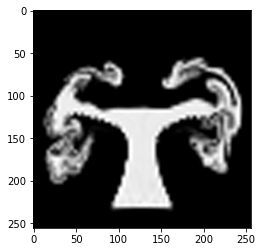
\includegraphics[scale=0.4]{superresolution/density_low.png}
		\caption{$Downsampled$}
	\end{subfigure}
	\begin{subfigure}{0.32\textwidth}
		\centering
		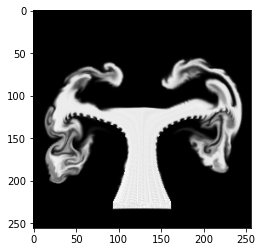
\includegraphics[scale=0.4]{superresolution/density_ref.png}
		\caption{$Reference$}
	\end{subfigure}
	\begin{subfigure}{0.32\textwidth}
		\centering
		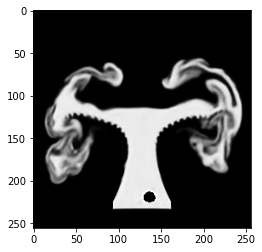
\includegraphics[scale=0.4]{superresolution/density_mse.png}
		\caption{$MSE$}
	\end{subfigure}
	\begin{subfigure}{0.32\textwidth}
		\centering
		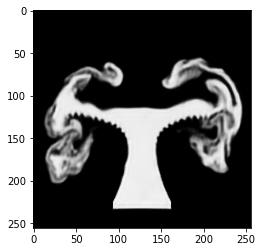
\includegraphics[scale=0.4]{superresolution/density_lsim.png}
		\caption{$LSiM$}
	\end{subfigure}
	\begin{subfigure}{0.32\textwidth}
		\centering
		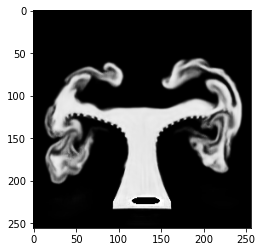
\includegraphics[scale=0.4]{superresolution/density_vgg.png}
		\caption{$VGG-16$}
	\end{subfigure}
	\begin{subfigure}{0.32\textwidth}
		\centering
		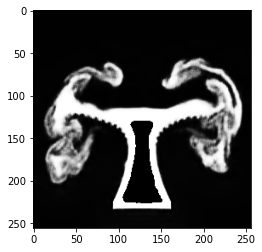
\includegraphics[scale=0.4]{superresolution/density_lpips.png}
		\caption{$Lpips$}
	\end{subfigure}
	\caption{Smoke density images reconstructions of super-resolution task }
	\label{super density}
\end{figure}

\begin{figure}
	\centering
	\begin{subfigure}{0.32\textwidth}
		\centering
		\includegraphics[scale=0.4]{superresolution/pressure_low.png}
		\caption{$Downsampled$}
	\end{subfigure}
	\begin{subfigure}{0.32\textwidth}
		\centering
		\includegraphics[scale=0.4]{superresolution/pressure_ref.png}
		\caption{$Reference$}
	\end{subfigure}
	\begin{subfigure}{0.32\textwidth}
		\centering
		\includegraphics[scale=0.4]{superresolution/pressure_mse.png}
		\caption{$MSE$}
	\end{subfigure}
	\begin{subfigure}{0.32\textwidth}
		\centering
		\includegraphics[scale=0.4]{superresolution/pressure_lsim.png}
		\caption{$LSiM$}
	\end{subfigure}
	\begin{subfigure}{0.32\textwidth}
		\centering
		\includegraphics[scale=0.4]{superresolution/pressure_vgg.png}
		\caption{$VGG-16$}
	\end{subfigure}
	\begin{subfigure}{0.32\textwidth}
		\centering
		\includegraphics[scale=0.4]{superresolution/pressure_lpips.png}
		\caption{$Lpips$}
	\end{subfigure}
	\caption{Smoke Pressure images reconstructions of super-resolution task}
	\label{super pressure}
\end{figure}

\begin{figure}
	\centering
	\begin{subfigure}{0.32\textwidth}
		\centering
		\includegraphics[scale=0.4]{superresolution/liquidvel_low.png}
		\caption{$Downsampled$}
	\end{subfigure}
	\begin{subfigure}{0.32\textwidth}
		\centering
		\includegraphics[scale=0.4]{superresolution/liquidvel_ref.png}
		\caption{$Reference$}
	\end{subfigure}
	\begin{subfigure}{0.32\textwidth}
		\centering
		\includegraphics[scale=0.4]{superresolution/liquidvel_mse.png}
		\caption{$MSE$}
	\end{subfigure}
	\begin{subfigure}{0.32\textwidth}
		\centering
		\includegraphics[scale=0.4]{superresolution/liquidvel_lsim.png}
		\caption{$LSiM$}
	\end{subfigure}
	\begin{subfigure}{0.32\textwidth}
		\centering
		\includegraphics[scale=0.4]{superresolution/liquidvel_vgg.png}
		\caption{$VGG-16$}
	\end{subfigure}
	\begin{subfigure}{0.32\textwidth}
		\centering
		\includegraphics[scale=0.4]{superresolution/liquidvel_lpips.png}
		\caption{$Lpips$}
	\end{subfigure}
	\caption{Liquid velocity images reconstructions of super-resolution task}
	\label{super liquid}
\end{figure}

\begin{figure}
	\centering
	\begin{subfigure}{0.32\textwidth}
		\centering
		\includegraphics[scale=0.5]{superresolution/l2.png}
		\caption{L2 evaluation}
	\end{subfigure}
	\begin{subfigure}{0.32\textwidth}
		\centering
		\includegraphics[scale=0.5]{superresolution/l1.png}
		\caption{L1 evaluation}
	\end{subfigure}
	\begin{subfigure}{0.32\textwidth}
		\centering
		\includegraphics[scale=0.5]{superresolution/mse.png}
		\caption{MSE evaluation}
	\end{subfigure}
	\begin{subfigure}{0.32\textwidth}
		\centering
		\includegraphics[scale=0.5]{superresolution/lsim.png}
		\caption{LSiM evaluation}
	\end{subfigure}
	\begin{subfigure}{0.32\textwidth}
		\centering
		\includegraphics[scale=0.5]{superresolution/ssim.png}
		\caption{SSIM evaluation}
	\end{subfigure}
	\begin{subfigure}{0.32\textwidth}
		\centering
		\includegraphics[scale=0.5]{superresolution/lpips.png}
		\caption{Lpips evaluation}
	\end{subfigure}
	\caption{Numerical evaluation of each metrics on test set of the super-resolution task}
	\label{super numeval}
\end{figure}
We train our ImageTransformNet based super-resolution model on the data combined by smoke and liquid data. Both smoke and liquid data consist of density, velocity and pressure images. We sample them all in gray scale hence only one channel.
We can see in terms of smoke density images(see figure \ref{super density}), every other metric has some artifacts within the plumes, while LSiM reconstructs the downsampled images well. This problem can be solved if we choose to train our model solely on the smoke density data. However the model will then lose its generality.
As for the liquid velocity images(see figure \ref{super liquid}), we can see that MSE generates a more blur image comparing to the others. Because MSE metric is prone to outliers so it tends to achieve a blur image to reduce the loss value. The other two metrics LSiM and Lpips, on the other hand, tend to generate a sharper image to approach the reference. In this case, VGG-16 metric achieves the best performance.

We also run the numerical evaluations(see figure \ref{super numeval}) on all the models we trained. We use 6 metrics to compute the distance between each model outputs and the references. According to the charts, we can tell that Lpips has the worst performance over all metrics, which is similar to the result of the autoencoder task. The other three metrics share the similar results in L2 and SSIM evaluation. VGG-16 achieves the best score in LSiM evaluation, LSiM itself achieves the second best and MSE the third. Overall VGG-16 has the best performance in terms of the numerical evaluations.


\begin{figure}
	\centering
	\begin{subfigure}{0.32\textwidth}
		\centering
		\includegraphics[scale=0.5]{superresolution/checkerboard_mse.png}
		\caption{MSE output}
	\end{subfigure}
	\begin{subfigure}{0.32\textwidth}
		\centering
		\includegraphics[scale=0.5]{superresolution/checkerboard_lsim.png}
		\caption{LSiM output}
	\end{subfigure}
	\begin{subfigure}{0.32\textwidth}
		\centering
		\includegraphics[scale=0.5]{superresolution/checkerboard_vgg.png}
		\caption{VGG-16 output}
	\end{subfigure}
	\begin{subfigure}{0.32\textwidth}
		\centering
		\includegraphics[scale=0.5]{superresolution/checkerboard_ref.png}
		\caption{Reference}
	\end{subfigure}
	\caption{Besides we have also tested the RGB channels model of ImageTransformNet on the density data. We can see when trained with LSiM metric, the output image has very obvious artifacts that tends to divide the images into 9 parts. This problem can be solved by sampling the images in gray scale and adopt the one channel ImageTransformNet model}
	\label{super rgb}
\end{figure}

We also test the karman flow data(see figure \ref{super karman}) from Solver in the Loop in the super-resolution model. 
\begin{figure}
	\centering
	\begin{subfigure}{0.32\textwidth}
		\centering
		\includegraphics[scale=0.5]{superresolution/karman_down.png}
		\caption{$Downsampled$}
	\end{subfigure}
	\begin{subfigure}{0.32\textwidth}
		\centering
		\includegraphics[scale=0.5]{superresolution/karman_ref.png}
		\caption{$Reference$}
	\end{subfigure}
	\begin{subfigure}{0.32\textwidth}
		\centering
		\includegraphics[scale=0.5]{superresolution/karman_mse.png}
		\caption{$MSE$}
	\end{subfigure}
	\begin{subfigure}{0.32\textwidth}
		\centering
		\includegraphics[scale=0.5]{superresolution/karman_lsim.png}
		\caption{$LSiM$}
	\end{subfigure}
	\begin{subfigure}{0.32\textwidth}
		\centering
		\includegraphics[scale=0.5]{superresolution/karman_vgg.png}
		\caption{$VGG-16$}
	\end{subfigure}
	\begin{subfigure}{0.32\textwidth}
		\centering
		\includegraphics[scale=0.5]{superresolution/karman_lpips.png}
		\caption{$Lpips$}
	\end{subfigure}
	\caption{karman flow images comparison}
	\label{super karman}
\end{figure}
The numerical evaluation is quite surprising(see figure \ref{super karman numeval}). Despite Lpips outputs have the closest color to the reference, it has the worst score over all the evaluations. LSiM achieves the best score in all evaluations. However intuitively, we can hardly tell the difference between the MSE, LSiM and VGG-16 outputs.
 
\begin{figure}
	\centering
	\begin{subfigure}{0.32\textwidth}
		\centering
		\includegraphics[scale=0.48]{superresolution/karman_eval_l2.png}
		\caption{L2 evaluation}
	\end{subfigure}
	\begin{subfigure}{0.32\textwidth}
		\centering
		\includegraphics[scale=0.48]{superresolution/karman_eval_l1.png}
		\caption{L1 evaluation}
	\end{subfigure}
	\begin{subfigure}{0.32\textwidth}
		\centering
		\includegraphics[scale=0.48]{superresolution/karman_eval_mse.png}
		\caption{MSE evaluation}
	\end{subfigure}
	\begin{subfigure}{0.32\textwidth}
		\centering
		\includegraphics[scale=0.48]{superresolution/karman_eval_lsim.png}
		\caption{LSiM evaluation}
	\end{subfigure}
	\begin{subfigure}{0.32\textwidth}
		\centering
		\includegraphics[scale=0.48]{superresolution/karman_eval_ssim.png}
		\caption{SSIM evaluation}
	\end{subfigure}
	\begin{subfigure}{0.32\textwidth}
		\centering
		\includegraphics[scale=0.48]{superresolution/karman_eval_lpips.png}
		\caption{Lpips evaluation}
	\end{subfigure}
	\caption{Numerical evaluation of each metrics on test set of the super-resolution task trained on karman flow data}
	\label{super karman numeval}
\end{figure}

\subsection{Solver in the loop}
After training lots of models on both buoyancy driven flow and the karman flow of different resolutions, we have following results. In terms of numerical evaluations, we compute the distance of various metrics(L1, L2, MSE, LSiM, SSIM, Lpips) between the simulation corrected by the models trained by different loss functions, and the down-sampled reference simulation. We compute the distance between each corresponding frames pair and compute their average as the result.

\paragraph{Karman flow}
From the comparisons from the figures, we can see that the source simulation(see figure \ref{sol karman high source}) deviates from the reference (see figure \ref{sol karman high ref}) after 1000 steps. Lpips (see figure \ref{sol karman high lpips}) obviously has the worst performance, the plume is shifting to the right and there are noticeable artifacts near the obstacle. MSE, LSiM and VGG-16(see figures \ref{sol karman high mse} , \ref{sol karman high lsim} , \ref{sol karman high vgg})  share similar outputs after step 1000.

In our numerical evaluations(see figure \ref{sol karman high numeval}), we only compare the simulation frames after step 1000 with their reference frames. We didn't compare the whole 1500 steps because we believe that considering all steps is not suitable since the reference images of the training only come from the latter 500 simulation steps. In terms of L1, L2 and MSE comparisons, we can see all corrected models have better scores than the source simulation. In the other evaluations, LSiM achieves overall the best score, followed by the VGG-16. MSE is not better than the source simulation, which is deviated from \citeauthor{um2020sol}'s work. We think the deviation may result from that we didn't choose a large multiple steps size\footnote{The multiple steps size is the number of the consecutive frames we focus on in one training step. It's similar to batch size, the larger the multiple steps size is, the more GPU memory it requires}, or a large training epoch. Still we prove that LSiM or VGG-16 outperform MSE in terms of this specific task.



\begin{figure}
	\centering
	\begin{subfigure}{0.32\textwidth}
		\centering
		\includegraphics[scale=0.49]{karmanflow/l2.png}
		\caption{L2 evaluation}
	\end{subfigure}
	\begin{subfigure}{0.32\textwidth}
		\centering
		\includegraphics[scale=0.49]{karmanflow/l1.png}
		\caption{L1 evaluation}
	\end{subfigure}
	\begin{subfigure}{0.32\textwidth}
		\centering
		\includegraphics[scale=0.49]{karmanflow/mse.png}
		\caption{MSE evaluation}
	\end{subfigure}
	\begin{subfigure}{0.32\textwidth}
		\centering
		\includegraphics[scale=0.49]{karmanflow/lsim.png}
		\caption{LSiM evaluation}
	\end{subfigure}
	\begin{subfigure}{0.32\textwidth}
		\centering
		\includegraphics[scale=0.49]{karmanflow/ssim.png}
		\caption{SSIM evaluation}
	\end{subfigure}
	\begin{subfigure}{0.32\textwidth}
		\centering
		\includegraphics[scale=0.49]{karmanflow/lpips.png}
		\caption{Lpips evaluation}
	\end{subfigure}
	\caption{Numerical evaluation of each metrics on test set with the reference}
	\label{sol karman high numeval}
\end{figure}

We also tested the karman flow on a lower resolution, whose simulation was running on a 64*64 domain.
The numerical evaluations(see figure \ref{sol karman low numeval}) are a little different from the training on a higher domain(see figure \ref{sol karman high numeval}). The outputs from all trained model(see figure \ref{sol karman low}) are intuitively similar. We only show the last frame of each model output including the reference and the source simulation, but we add the respective gifs as the hyperlink in the caption.
We can see on a lower domain, Lpips metric outperform the others, while LSiM is the worst over all 4 metrics. However all the metrics outperform the source simulation in terms of MSE, L2, SSIM and Lpips evaluation, especially in Lpips and L2(MSE) evaluation. Every corrected model has made a strong difference comparing to the source simulation.  


\begin{figure}
	\centering
	\begin{subfigure}{0.32\textwidth}
		\centering
		\includegraphics[scale=0.49]{karman_low/numeval_l2.png}
		\caption{L2 evaluation}
	\end{subfigure}
	\begin{subfigure}{0.32\textwidth}
		\centering
		\includegraphics[scale=0.49]{karman_low/numeval_l1.png}
		\caption{L1 evaluation}
	\end{subfigure}
	\begin{subfigure}{0.32\textwidth}
		\centering
		\includegraphics[scale=0.49]{karman_low/numeval_mse.png}
		\caption{MSE evaluation}
	\end{subfigure}
	\begin{subfigure}{0.32\textwidth}
		\centering
		\includegraphics[scale=0.49]{karman_low/numeval_lsim.png}
		\caption{LSiM evaluation}
	\end{subfigure}
	\begin{subfigure}{0.32\textwidth}
		\centering
		\includegraphics[scale=0.49]{karman_low/numeval_ssim.png}
		\caption{SSIM evaluation}
	\end{subfigure}
	\begin{subfigure}{0.32\textwidth}
		\centering
		\includegraphics[scale=0.49]{karman_low/numeval_lpips.png}
		\caption{Lpips evaluation}
	\end{subfigure}
	\caption{Numerical evaluation of each metrics on test set with the reference on the 64*64 domain}
	\label{sol karman low numeval}
\end{figure}

\paragraph{Buoyancy driven flow}
We first run the evaluation on a test set of the buoyancy driven flow on the higher domain(128*128). We can see from the simulation images, the corrected simulation(see figures \ref{sol buoyancy high lsim}, \ref{sol buoyancy high mse}, \ref{sol buoyancy high vgg}) can hardly approach the shape of the reference images(see figure \ref{sol buoyancy high ref}) Only the corrected simulation trained by Lpips(see figure \ref{sol buoyancy high lpips}) shares a little similarity with the reference. The same concept is also revealed in the numerical evaluation of these models(see figure \ref{sol buoyancy high numeval}). Except Lpips, other metrics can not even outperform the uncorrected source simulation. 

For completeness we also turn to the buoyancy driven flow on the lower domain(64*64)(see figure \ref{sol buoyancy low}), the result is similar or even worse. We can see from the numerical evaluation(see figure \ref{sol buoyancy low numeval}), except for the LSiM evaluation, the source simulation outperform all the corrected simulation. However, if we only look at the comparisons between the corrected simulation, we can see that generally LSiM and VGG-16 metrics achieve better scores than MSE.


\begin{figure}
	\centering
	\begin{subfigure}{0.32\textwidth}
		\centering
		\includegraphics[scale=0.48]{buoyancy_test/l2.png}
		\caption{L2 evaluation}
	\end{subfigure}
	\begin{subfigure}{0.32\textwidth}
		\centering
		\includegraphics[scale=0.48]{buoyancy_test/l1.png}
		\caption{L1 evaluation}
	\end{subfigure}
	\begin{subfigure}{0.32\textwidth}
		\centering
		\includegraphics[scale=0.48]{buoyancy_test/mse.png}
		\caption{MSE evaluation}
	\end{subfigure}
	\begin{subfigure}{0.32\textwidth}
		\centering
		\includegraphics[scale=0.48]{buoyancy_test/lsim.png}
		\caption{LSiM evaluation}
	\end{subfigure}
	\begin{subfigure}{0.32\textwidth}
		\centering
		\includegraphics[scale=0.48]{buoyancy_test/ssim.png}
		\caption{SSIM evaluation}
	\end{subfigure}
	\begin{subfigure}{0.32\textwidth}
		\centering
		\includegraphics[scale=0.48]{buoyancy_test/lpips.png}
		\caption{Lpips evaluation}
	\end{subfigure}
	\caption{Numerical evaluation of each metrics on test set of buoyancy driven flow with the domain resolution of 128*128 with Renold's number=2.5e5}
	\label{sol buoyancy high numeval}
		\end{figure}
	
	
	
	
	\begin{figure}
		\centering
		\begin{subfigure}{0.32\textwidth}
			\centering
			\includegraphics[scale=0.49]{buoyancy_low/l2.png}
			\caption{L2 evaluation}
		\end{subfigure}
		\begin{subfigure}{0.32\textwidth}
			\centering
			\includegraphics[scale=0.49]{buoyancy_low/l1.png}
			\caption{L1 evaluation}
		\end{subfigure}
		\begin{subfigure}{0.32\textwidth}
			\centering
			\includegraphics[scale=0.49]{buoyancy_low/mse_eval.png}
			\caption{MSE evaluation}
		\end{subfigure}
		\begin{subfigure}{0.32\textwidth}
			\centering
			\includegraphics[scale=0.49]{buoyancy_low/lsim_eval.png}
			\caption{LSiM evaluation}
		\end{subfigure}
		\begin{subfigure}{0.32\textwidth}
			\centering
			\includegraphics[scale=0.49]{buoyancy_low/ssim.png}
			\caption{SSIM evaluation}
		\end{subfigure}
		\begin{subfigure}{0.32\textwidth}
			\centering
			\includegraphics[scale=0.49]{buoyancy_low/lpips_eval.png}
			\caption{Lpips evaluation}
		\end{subfigure}
		\caption{Numerical evaluation of each metrics on test set with the reference on the 64*64 domain}
		\label{sol buoyancy low numeval}
	\end{figure}

\subsection{Time cost evaluation}
In this evaluation we combine the SOL model and the super-resolution model for karman flow on the domain of 64*64. We want to demonstrate the time cost and the quality difference between
\begin{itemize}
	\item running  the pure physical simulation on the higher domain, without any deep learning models involved (see figure \ref{timecost ref})
	\item running first the corrected physical simulation on the lower domain by the pretrained SOL model and then apply the super-resolution model to the same resolution of the higher domain (see figure \ref{timecost out})
\end{itemize}
The outputs are satisfying. We can see barely any artifacts from the outputs and the simulation is similar to the reference. We average the time cost of generating the 2 simulations. We have 14 min 6 sec on average for generating 1500 images of the reference(see figure \ref{timecost ref}) and 4 min 23 sec for generating the second simulation(see figure \ref{timecost out}). The time cost reduced by 70\% if we choose to generate a corrected low-resolution simulation and adopt the super-resolution model rather than performing the pure physical simulation on the higher-resolution domain. Meanwhile, the outputs are similar in terms of both the quality and the shape of the plumes.  

\begin{figure}
	\centering
	\begin{subfigure}{0.18\textwidth}
		\centering
		\includegraphics[scale=0.3]{timecost/ref250.png}
		\caption{$t=250$}
	\end{subfigure}
	\begin{subfigure}{0.18\textwidth}
		\centering
		\includegraphics[scale=0.3]{timecost/ref500.png}
		\caption{$t=500$}
	\end{subfigure}
	\begin{subfigure}{0.18\textwidth}
		\centering
		\includegraphics[scale=0.3]{timecost/ref1000.png}
		\caption{$t=1000$}
	\end{subfigure}
	\begin{subfigure}{0.18\textwidth}
		\centering
		\includegraphics[scale=0.3]{timecost/ref1250.png}
		\caption{$t=1250$}
	\end{subfigure}
	\begin{subfigure}{0.18\textwidth}
		\centering
		\includegraphics[scale=0.3]{timecost/ref1499.png}
		\caption{$t=1499$}
	\end{subfigure}
	\caption{Karman flow reference simulation \href{https://github.com/w191444052/sol-data/blob/master/sol\%2Bsuperresolution/ref.gif}{\textbf{gif here}}}
	\label{timecost ref}
\end{figure}

\begin{figure}
	\centering
	\begin{subfigure}{0.18\textwidth}
		\centering
		\includegraphics[scale=0.3]{timecost/low250.png}
		\caption{$t=250$}
	\end{subfigure}
	\begin{subfigure}{0.18\textwidth}
		\centering
		\includegraphics[scale=0.3]{timecost/low500.png}
		\caption{$t=500$}
	\end{subfigure}
	\begin{subfigure}{0.18\textwidth}
		\centering
		\includegraphics[scale=0.3]{timecost/low1000.png}
		\caption{$t=1000$}
	\end{subfigure}
	\begin{subfigure}{0.18\textwidth}
		\centering
		\includegraphics[scale=0.3]{timecost/low1250.png}
		\caption{$t=1250$}
	\end{subfigure}
	\begin{subfigure}{0.18\textwidth}
		\centering
		\includegraphics[scale=0.3]{timecost/low1499.png}
		\caption{$t=1499$}
	\end{subfigure}
	\caption{Karman flow low simulation + SOL model + super-resolution model \href{https://github.com/w191444052/sol-data/blob/master/sol\%2Bsuperresolution/sol\%2Bsuperresolution_output.gif}{\textbf{gif here}}}
	\label{timecost out}
\end{figure}

\section{Limitations}
\paragraph{Autoencoder} We think the network we build for the autoencoder task is rather small and shallow. It only consists of 4 feature extraction layers, so the distance between using perceptual losses and traditional loss functions may not be explicitly revealed. We only choose to train the model that handles the gray scale images, while in more complicated use cases there could be fluid images with RGB channels. For such conditions we need to train a more complicated model.
\paragraph{Super-resolution} When we use the data sets that consist all the density, velocity and pressure images, the model seems very hard to generalize for such data sets. We can notice lots of artifacts within the density reconstruction plumes. We might need to add some regularization to the network to let the model apply to the data sets with high variations. We also tested the RGB-channel version of the network. The outputs of the network still consist of some artifacts. We can see vaguely that the outputs are divided into 9 parts, we may need to redesign the network to eliminate such artifacts.
\paragraph{Solver in the Loop}Due to the GPU memory limitation(we used a GTX 1080Ti with 11GiB of memory to train the SOL  model), we are unable to choose a higher multiple steps size to train the model.\footnote{The multiple steps size is the number of the consecutive frames we focus on in one training step. It's similar to batch size, the larger the multiple steps size is, the more GPU memory it requires}. We choose the multi step size in both buoyancy driven flow and karman flow as 8. \citeauthor{um2020sol} used some similar multi step size for karman flow, however 128 for the buoyancy driven flow. We think that the reason why our buoyancy driven flow is not working as expected may come from that we choose a too small multi step size.




%------- chapter 6 -------

\chapter{Conclusion}
\section{Future work}
We can try to extend the model of super-resolution and autoencoder to the RGB channel and test on fluid data with RGB-channels. Adding more regularization to the training would also be an improvement.

For the Solver in the Loop model, we can choose to upsample the model outputs and compare them with the reference instead of downsampling the reference to compare with the model outputs. In such way, we do not need to pad our low-resolution domain to suit the minimal input size of the LSiM model. Besides, we can consider all the 1500 simulation steps of karman flow and enlarge the simulation multi steps and data sets to train a more general model. We can also include more fluid simulation types(not just karman flow and buoyancy driven flow) to the data sets and train them on a more higher-resolution domain to see whether the distance between MSE and perceptual losses becomes bigger.

Moreover we can try to compare the performance of perceptual losses in other tasks, e.g. inpaintings\cite{DBLP:journals/corr/abs-1712-03111}, style transfer for the fluids\cite{kim2020lagrangian} etc. Especially in \cite{kim2020lagrangian}, the data sets are fluids with RGB-channels. We can try out different perceptual loss functions for computing the loss of shapes and the loss of styles, which is similar to\cite{johnson2016perceptual}'s model architecture(see figure \ref{vgg-16-perceptual}).
\section{Summary}
In this thesis, we successfully proved the advantage of using perceptual losses in some fluid simulation related tasks. However, in some tasks, using perceptual losses is not necessarily better than using traditional loss functions. There is no one dominant perceptual loss function for every task. For the super-resolution model(see figure \ref{super numeval}) on the smoke and liquid data sets, the VGG-16 demonstrates the best performance over all the 4 metrics. While for the same model on the karman flow data sets, LSiM achieves the best score(see figure \ref{super karman numeval}). 
In the super-resolution task, we also notice that the distance between using MSE and perceptual losses is smaller when we train the model that handles gray scale images(see figure \ref{super density}) rather than RGB-channel images(see figure \ref{super rgb}). The similar result also appears in the Solver in the Loop task. After running tests on both the karman flow and buoyancy driven flow, we can see that the perceptual losses tend to perform better in more complicated conditions. Both for the karman flow(see figures \ref{sol karman high numeval} vs \ref{sol karman low numeval}) and buoyancy driven flow(see figures \ref{sol buoyancy high numeval} vs \ref{sol buoyancy low numeval}), the numerical distance between using perceptual losses and MSE is bigger when running the simulation on the higher domain. Similarly, if we compare the higher resolution simulation between karman flow and buoyancy driven flow(see figures \ref{sol karman high numeval} vs \ref{sol buoyancy high numeval}, \ref{sol karman low numeval} vs \ref{sol buoyancy low numeval}), we can tell that the numerical distance between using perceptual losses and MSE is bigger when running the buoyancy driven flow simulation. Despite the fact that some of the corrected simulations are not even better than the source simulation, we can still judge in terms of loss functions, that perceptual losses tend to perform better under more complicated conditions. 




\appendix

\begin{figure}[p]
	\centering
	\begin{subfigure}{0.18\textwidth}
		\centering
		\includegraphics[scale=0.5]{karmanflow/ref_density_000250.png}
		\caption{$t=250$}
	\end{subfigure}
	\begin{subfigure}{0.18\textwidth}
		\centering
		\includegraphics[scale=0.5]{karmanflow/ref_density_000500.png}
		\caption{$t=500$}
	\end{subfigure}
	\begin{subfigure}{0.18\textwidth}
		\centering
		\includegraphics[scale=0.5]{karmanflow/ref_density_001000.png}
		\caption{$t=1000$}
	\end{subfigure}
	\begin{subfigure}{0.18\textwidth}
		\centering
		\includegraphics[scale=0.5]{karmanflow/ref_density_001250.png}
		\caption{$t=1250$}
	\end{subfigure}
	\begin{subfigure}{0.18\textwidth}
		\centering
		\includegraphics[scale=0.5]{karmanflow/ref_density_001499.png}
		\caption{$t=1499$}
	\end{subfigure}
	\caption{Karman flow reference simulation \href{https://github.com/w191444052/sol-data/blob/master/karman_high/ref.gif}{\bf{gif here}}}
	\label{sol karman high ref}
\end{figure}

\begin{figure}
	\centering
	\begin{subfigure}{0.18\textwidth}
		\centering
		\includegraphics[scale=0.5]{karmanflow/source_density_000250.png}
		\caption{$t=250$}
	\end{subfigure}
	\begin{subfigure}{0.18\textwidth}
		\centering
		\includegraphics[scale=0.5]{karmanflow/source_density_000500.png}
		\caption{$t=500$}
	\end{subfigure}
	\begin{subfigure}{0.18\textwidth}
		\centering
		\includegraphics[scale=0.5]{karmanflow/source_density_001000.png}
		\caption{$t=1000$}
	\end{subfigure}
	\begin{subfigure}{0.18\textwidth}
		\centering
		\includegraphics[scale=0.5]{karmanflow/source_density_001250.png}
		\caption{$t=1250$}
	\end{subfigure}
	\begin{subfigure}{0.18\textwidth}
		\centering
		\includegraphics[scale=0.5]{karmanflow/source_density_001499.png}
		\caption{$t=1499$}
	\end{subfigure}
	\caption{Karman flow source simulation without correction  \href{https://github.com/w191444052/sol-data/blob/master/karman_high/source.gif}{\bf{gif here}}}
	\label{sol karman high source}
\end{figure}

\begin{figure}
	\centering
	\begin{subfigure}{0.18\textwidth}
		\centering
		\includegraphics[scale=0.5]{karmanflow/mse_density_000250.png}
		\caption{$t=250$}
	\end{subfigure}
	\begin{subfigure}{0.18\textwidth}
		\centering
		\includegraphics[scale=0.5]{karmanflow/mse_density_000500.png}
		\caption{$t=500$}
	\end{subfigure}
	\begin{subfigure}{0.18\textwidth}
		\centering
		\includegraphics[scale=0.5]{karmanflow/mse_density_001000.png}
		\caption{$t=1000$}
	\end{subfigure}
	\begin{subfigure}{0.18\textwidth}
		\centering
		\includegraphics[scale=0.5]{karmanflow/mse_density_001250.png}
		\caption{$t=1250$}
	\end{subfigure}
	\begin{subfigure}{0.18\textwidth}
		\centering
		\includegraphics[scale=0.5]{karmanflow/mse_density_001499.png}
		\caption{$t=1499$}
	\end{subfigure}
	\caption{Karman flow simulation trained with MSE on the 128*128 domain \href{https://github.com/w191444052/sol-data/blob/master/karman_high/mse.gif}{\bf{gif here}}}
	\label{sol karman high mse}
\end{figure}

\begin{figure}
	\centering
	\begin{subfigure}{0.18\textwidth}
		\centering
		\includegraphics[scale=0.5]{karmanflow/lsim_density_000250.png}
		\caption{$t=250$}
	\end{subfigure}
	\begin{subfigure}{0.18\textwidth}
		\centering
		\includegraphics[scale=0.5]{karmanflow/lsim_density_000500.png}
		\caption{$t=500$}
	\end{subfigure}
	\begin{subfigure}{0.18\textwidth}
		\centering
		\includegraphics[scale=0.5]{karmanflow/lsim_density_001000.png}
		\caption{$t=1000$}
	\end{subfigure}
	\begin{subfigure}{0.18\textwidth}
		\centering
		\includegraphics[scale=0.5]{karmanflow/lsim_density_001250.png}
		\caption{$t=1250$}
	\end{subfigure}
	\begin{subfigure}{0.18\textwidth}
		\centering
		\includegraphics[scale=0.5]{karmanflow/lsim_density_001499.png}
		\caption{$t=1499$}
	\end{subfigure}
	\caption{Karman flow simulation trained with LSiM on the 128*128 domain \href{https://github.com/w191444052/sol-data/blob/master/karman_high/lsim.gif}{\bf{gif here}}}
	\label{sol karman high lsim}
\end{figure}

\begin{figure}
	\centering
	\begin{subfigure}{0.18\textwidth}
		\centering
		\includegraphics[scale=0.5]{karmanflow/lpips_density_000250.png}
		\caption{$t=250$}
	\end{subfigure}
	\begin{subfigure}{0.18\textwidth}
		\centering
		\includegraphics[scale=0.5]{karmanflow/lpips_density_000500.png}
		\caption{$t=500$}
	\end{subfigure}
	\begin{subfigure}{0.18\textwidth}
		\centering
		\includegraphics[scale=0.5]{karmanflow/lpips_density_001000.png}
		\caption{$t=1000$}
	\end{subfigure}
	\begin{subfigure}{0.18\textwidth}
		\centering
		\includegraphics[scale=0.5]{karmanflow/lpips_density_001250.png}
		\caption{$t=1250$}
	\end{subfigure}
	\begin{subfigure}{0.18\textwidth}
		\centering
		\includegraphics[scale=0.5]{karmanflow/lpips_density_001499.png}
		\caption{$t=1499$}
	\end{subfigure}
	\caption{Karman flow simulation with Lpips on the 128*128 domain\href{https://github.com/w191444052/sol-data/blob/master/karman_high/lpips.gif}{\bf{gif here}}}
	\label{sol karman high lpips}
\end{figure}

\begin{figure}
	\centering
	\begin{subfigure}{0.18\textwidth}
		\centering
		\includegraphics[scale=0.5]{karmanflow/vgg_density_000250.png}
		\caption{$t=250$}
	\end{subfigure}
	\begin{subfigure}{0.18\textwidth}
		\centering
		\includegraphics[scale=0.5]{karmanflow/vgg_density_000500.png}
		\caption{$t=500$}
	\end{subfigure}
	\begin{subfigure}{0.18\textwidth}
		\centering
		\includegraphics[scale=0.5]{karmanflow/vgg_density_001000.png}
		\caption{$t=1000$}
	\end{subfigure}
	\begin{subfigure}{0.18\textwidth}
		\centering
		\includegraphics[scale=0.5]{karmanflow/vgg_density_001250.png}
		\caption{$t=1250$}
	\end{subfigure}
	\begin{subfigure}{0.18\textwidth}
		\centering
		\includegraphics[scale=0.5]{karmanflow/vgg_density_001499.png}
		\caption{$t=1499$}
	\end{subfigure}
	\caption{Karman flow simulation trained with VGG-16 on the 128*128 domain \href{https://github.com/w191444052/sol-data/blob/master/karman_high/vgg.gif}{\bf{gif here}}}
	\label{sol karman high vgg}
\end{figure}

\begin{figure}
	\centering
	\begin{subfigure}{0.32\textwidth}
		\centering
		\includegraphics[scale=0.5]{karman_low/ref}
		\caption{Reference}
	\end{subfigure}
	\begin{subfigure}{0.32\textwidth}
		\centering
		\includegraphics[scale=0.5]{karman_low/source}
		\caption{Source}
	\end{subfigure}
	\begin{subfigure}{0.32\textwidth}
		\centering
		\includegraphics[scale=0.5]{karman_low/mse}
		\caption{MSE}
	\end{subfigure}
	\begin{subfigure}{0.32\textwidth}
		\centering
		\includegraphics[scale=0.5]{karman_low/lsim}
		\caption{LSiM}
	\end{subfigure}
	\begin{subfigure}{0.32\textwidth}
		\centering
		\includegraphics[scale=0.5]{karman_low/vgg}
		\caption{VGG-16}
	\end{subfigure}
	\begin{subfigure}{0.32\textwidth}
		\centering
		\includegraphics[scale=0.5]{karman_low/lpips}
		\caption{Lpips}
	\end{subfigure}
	\caption{Karman flow simulation trained with each metric on the 64*64 domain comparing with the reference \href{https://github.com/w191444052/sol-data/tree/master/karman_low}{\bf{all gifs here}}}
	\label{sol karman low}
\end{figure}

\begin{figure}
	\centering
	\begin{subfigure}{0.18\textwidth}
		\centering
		\includegraphics[scale=0.28]{buoyancy_test/dens_000050_ref.png}
		\caption{$t=50$}
	\end{subfigure}
	\begin{subfigure}{0.18\textwidth}
		\centering
		\includegraphics[scale=0.28]{buoyancy_test/dens_000100_ref.png}
		\caption{$t=100$}
	\end{subfigure}
	\begin{subfigure}{0.18\textwidth}
		\centering
		\includegraphics[scale=0.28]{buoyancy_test/dens_000150_ref.png}
		\caption{$t=150$}
	\end{subfigure}
	\begin{subfigure}{0.18\textwidth}
		\centering
		\includegraphics[scale=0.28]{buoyancy_test/dens_000200_ref.png}
		\caption{$t=200$}
	\end{subfigure}
	\begin{subfigure}{0.18\textwidth}
		\centering
		\includegraphics[scale=0.28]{buoyancy_test/dens_000249_ref.png}
		\caption{$t=250$}
	\end{subfigure}
	\caption{Reference simulation of buoyancy driven flow on the 128*128 domain \href{https://github.com/w191444052/sol-data/blob/master/buoyancy_high/ref.gif}{\bf{gif here}}}
	\label{sol buoyancy high ref}
\end{figure}

\begin{figure}
	\centering
	\begin{subfigure}{0.18\textwidth}
		\centering
		\includegraphics[scale=0.56]{buoyancy_test/dens_000050_src.png}
		\caption{$t=50$}
	\end{subfigure}
	\begin{subfigure}{0.18\textwidth}
		\centering
		\includegraphics[scale=0.56]{buoyancy_test/dens_000100_src.png}
		\caption{$t=100$}
	\end{subfigure}
	\begin{subfigure}{0.18\textwidth}
		\centering
		\includegraphics[scale=0.56]{buoyancy_test/dens_000150_src.png}
		\caption{$t=150$}
	\end{subfigure}
	\begin{subfigure}{0.18\textwidth}
		\centering
		\includegraphics[scale=0.56]{buoyancy_test/dens_000200_src.png}
		\caption{$t=200$}
	\end{subfigure}
	\begin{subfigure}{0.18\textwidth}
		\centering
		\includegraphics[scale=0.56]{buoyancy_test/dens_000249_src.png}
		\caption{$t=250$}
	\end{subfigure}
	\caption{Source simulation of buoyancy driven flow on the 128*128 domain \href{https://github.com/w191444052/sol-data/blob/master/buoyancy_high/source.gif}{\bf{gif here}}}
	\label{sol buoyancy high source}
\end{figure}

\begin{figure}
	\centering
	\begin{subfigure}{0.18\textwidth}
		\centering
		\includegraphics[scale=0.56]{buoyancy_test/dens_000050_lsim.png}
		\caption{$t=50$}
	\end{subfigure}
	\begin{subfigure}{0.18\textwidth}
		\centering
		\includegraphics[scale=0.56]{buoyancy_test/dens_000100_lsim.png}
		\caption{$t=100$}
	\end{subfigure}
	\begin{subfigure}{0.18\textwidth}
		\centering
		\includegraphics[scale=0.56]{buoyancy_test/dens_000150_lsim.png}
		\caption{$t=150$}
	\end{subfigure}
	\begin{subfigure}{0.18\textwidth}
		\centering
		\includegraphics[scale=0.56]{buoyancy_test/dens_000200_lsim.png}
		\caption{$t=200$}
	\end{subfigure}
	\begin{subfigure}{0.18\textwidth}
		\centering
		\includegraphics[scale=0.56]{buoyancy_test/dens_000249_lsim.png}
		\caption{$t=250$}
	\end{subfigure}
	\caption{buoyancy driven flow simulation trained with LSiM on the 128*128 domain \href{https://github.com/w191444052/sol-data/blob/master/buoyancy_high/lsim.gif}{\bf{gif here}}}
	\label{sol buoyancy high lsim}
\end{figure}

\begin{figure}
	\centering
	\begin{subfigure}{0.18\textwidth}
		\centering
		\includegraphics[scale=0.56]{buoyancy_test/dens_000050_mse.png}
		\caption{$t=50$}
	\end{subfigure}
	\begin{subfigure}{0.18\textwidth}
		\centering
		\includegraphics[scale=0.56]{buoyancy_test/dens_000100_mse.png}
		\caption{$t=100$}
	\end{subfigure}
	\begin{subfigure}{0.18\textwidth}
		\centering
		\includegraphics[scale=0.56]{buoyancy_test/dens_000150_mse.png}
		\caption{$t=150$}
	\end{subfigure}
	\begin{subfigure}{0.18\textwidth}
		\centering
		\includegraphics[scale=0.56]{buoyancy_test/dens_000200_mse.png}
		\caption{$t=200$}
	\end{subfigure}
	\begin{subfigure}{0.18\textwidth}
		\centering
		\includegraphics[scale=0.56]{buoyancy_test/dens_000249_mse.png}
		\caption{$t=250$}
	\end{subfigure}
	\caption{Buoyancy driven flow simulation trained with MSE on the 128*128 domain \href{https://github.com/w191444052/sol-data/blob/master/buoyancy_high/mse.gif}{\bf{gif here}}}
	\label{sol buoyancy high mse}
\end{figure}

\begin{figure}
	\centering
	\begin{subfigure}{0.18\textwidth}
		\centering
		\includegraphics[scale=0.56]{buoyancy_test/dens_000050_vgg.png}
		\caption{$t=50$}
	\end{subfigure}
	\begin{subfigure}{0.18\textwidth}
		\centering
		\includegraphics[scale=0.56]{buoyancy_test/dens_000100_vgg.png}
		\caption{$t=100$}
	\end{subfigure}
	\begin{subfigure}{0.18\textwidth}
		\centering
		\includegraphics[scale=0.56]{buoyancy_test/dens_000150_vgg.png}
		\caption{$t=150$}
	\end{subfigure}
	\begin{subfigure}{0.18\textwidth}
		\centering
		\includegraphics[scale=0.56]{buoyancy_test/dens_000200_vgg.png}
		\caption{$t=200$}
	\end{subfigure}
	\begin{subfigure}{0.18\textwidth}
		\centering
		\includegraphics[scale=0.56]{buoyancy_test/dens_000249_vgg.png}
		\caption{$t=250$}
	\end{subfigure}
	\caption{Buoyancy driven flow simulation trained with VGG-16 on the 128*128 domain \href{https://github.com/w191444052/sol-data/blob/master/buoyancy_high/vgg.gif}{\bf{gif here}}}
	\label{sol buoyancy high vgg}
\end{figure}

\begin{figure}
	\centering
	\begin{subfigure}{0.18\textwidth}
		\centering
		\includegraphics[scale=0.56]{buoyancy_test/dens_000050_lpips.png}
		\caption{$t=50$}
	\end{subfigure}
	\begin{subfigure}{0.18\textwidth}
		\centering
		\includegraphics[scale=0.56]{buoyancy_test/dens_000100_lpips.png}
		\caption{$t=100$}
	\end{subfigure}
	\begin{subfigure}{0.18\textwidth}
		\centering
		\includegraphics[scale=0.56]{buoyancy_test/dens_000150_lpips.png}
		\caption{$t=150$}
	\end{subfigure}
	\begin{subfigure}{0.18\textwidth}
		\centering
		\includegraphics[scale=0.56]{buoyancy_test/dens_000200_lpips.png}
		\caption{$t=200$}
	\end{subfigure}
	\begin{subfigure}{0.18\textwidth}
		\centering
		\includegraphics[scale=0.56]{buoyancy_test/dens_000249_lpips.png}
		\caption{$t=250$}
	\end{subfigure}
	\caption{Buoyancy driven flow simulation trained with lpips on the 128*128 domain \href{https://github.com/w191444052/sol-data/blob/master/buoyancy_high/lpips.gif}{\bf{gif here}}}
	\label{sol buoyancy high lpips}
\end{figure}

	\begin{figure}
	\centering
	\begin{subfigure}{0.32\textwidth}
		\centering
		\includegraphics[scale=0.5]{buoyancy_low/ref}
		\caption{Reference at $t=149$}
	\end{subfigure}
	\begin{subfigure}{0.32\textwidth}
		\centering
		\includegraphics[scale=0.5]{buoyancy_low/source}
		\caption{Source at $t=149$}
	\end{subfigure}
	\begin{subfigure}{0.32\textwidth}
		\centering
		\includegraphics[scale=0.5]{buoyancy_low/mse}
		\caption{MSE at $t=149$}
	\end{subfigure}
	\begin{subfigure}{0.32\textwidth}
		\centering
		\includegraphics[scale=0.5]{buoyancy_low/lsim}
		\caption{LSiM at $t=149$}
	\end{subfigure}
	\begin{subfigure}{0.32\textwidth}
		\centering
		\includegraphics[scale=0.5]{buoyancy_low/vgg}
		\caption{VGG-16 at $t=149$}
	\end{subfigure}
	\begin{subfigure}{0.32\textwidth}
		\centering
		\includegraphics[scale=0.5]{buoyancy_low/lpips}
		\caption{Lpips at $t=149$}
	\end{subfigure}
	\caption{Buoyancy driven flow simulation trained with each metric on the 64*64 domain comparing with the reference and the source \href{https://github.com/w191444052/sol-data/tree/master/buoyancy_low}{\bf{all gifs here}}}
	\label{sol buoyancy low}
\end{figure}

%\textit{Note: If you have large models, additional evaluation data like questionnaires or non summarized results, put them into the appendix.}


\clearpage

\clearpage

\clearpage

\bibliography{thesis}
%\bibliographystyle{alpha}
\bibliographystyle{unsrtnat}

\end{document}
